\documentclass[10pt, twocolumn, twoside]{article}
\usepackage[top=1.2in, bottom=0.7in, left=0.7in, right=0.7in]{geometry}
\usepackage{amsmath}
\usepackage{amsthm}
\usepackage{amssymb}
\usepackage{placeins}
\usepackage{marvosym}
\usepackage[usenames,dvipsnames,table]{xcolor}
\usepackage{colortbl}
\usepackage{booktabs}
\usepackage{graphicx}
\usepackage{framed}
\usepackage{setspace}
\usepackage{xspace}
\usepackage[labelfont=bf]{caption}
\usepackage{verbatim}
\usepackage{paralist}
\usepackage{algorithm}
\usepackage{algpseudocode}
\usepackage{wrapfig}
\usepackage[font=footnotesize,labelfont=bf,justification=justified,singlelinecheck=false]{caption}
\usepackage{titlesec}
\usepackage{natbib}
\usepackage{longtable}
\usepackage{tabularx}
\usepackage{tabulary}
\usepackage{multirow}
\usepackage{lipsum}
\usepackage{mathpazo}
\usepackage{authblk}
\usepackage{nameref}
\usepackage{cancel}
\usepackage{commath}
\usepackage{xspace}
\usepackage{dsfont}
\usepackage{cuted}
\usepackage{fancyhdr}
\usepackage{hyperref}
\usepackage{longtable}
\usepackage{lineno}
\usepackage{graphicx}
\usepackage{movie15}
\linenumbers
\setcounter{secnumdepth}{0}

% bib
\setcitestyle{aysep={}}
\renewcommand{\bibsection}{\section*{\normalsize References}}
\setlength{\bibsep}{0pt plus 0.3ex}

% hyperref setup
\hypersetup{
  colorlinks = true,
  linkcolor = {blue},
  citecolor = {blue}
}

% distance between columns
\setlength{\columnsep}{6ex}

% section rules
\titleformat{\paragraph}[runin]
{\normalfont\itshape}
{\theparagraph}{}{\noindent}[.---]

\titlespacing{\paragraph}{0pt}{3.25ex plus 1ex minus .2ex}{0em}

\titleformat{\section}
  {\centering\scshape}{\thesection}{1em}{}

\titleformat{\subsection}
  {\centering\itshape}{\thesubsection}{1em}{}

% bibliography settings

% other stuff?
\setlength\bigstrutjot{3pt}
\makeatletter
\newlength\mylena
\newlength\mylenb
\newcommand\mystrut[1][2]{%
    \setlength\mylena{#1\ht\@arstrutbox}%
    \setlength\mylenb{#1\dp\@arstrutbox}%
    \rule[\mylenb]{0pt}{\mylena}}
\makeatother


\newcommand{\opensupplement}{

    \setcounter{figure}{0}

    \renewcommand{\thefigure}{S\thechapter.\arabic{figure}}
}

\newcommand{\closesupplement}{%

        \setcounter{figure}{0}
    \renewcommand{\thefigure}{\thechapter.\arabic{figure}}
     }

\hyphenation{dis-ser-ta-tion blue-print man-u-script pre-par-ing fra-me-work bayes-ian bra-nch} %add hyphenation rules for words TeX doesn't know


%%redefine longtable
%\makeatletter
%\let\oldlt\longtable
%\let\endoldlt\endlongtable
%\def\longtable{\@ifnextchar[\longtable@i \longtable@ii}
%\def\longtable@i[#1]{\begin{figure}[t]
%\onecolumn
%\begin{minipage}{0.5\textwidth}
%\oldlt[#1]
%}
%\def\longtable@ii{\begin{figure}[t]
%\onecolumn
%\begin{minipage}{0.5\textwidth}
%\oldlt
%}
%\def\endlongtable{\endoldlt
%\end{minipage}
%\twocolumn
%\end{figure}}
%\makeatother

% header
\pagestyle{fancy}
\fancyhf{}
\fancyhead[RO,LE]{\thepage}
\fancyhead[C]{\scshape VETR ET AL. --- HUMAN POPULATION HISTORY FROM DISCRETE DENTAL TRAITS}

% Title %

\title{\vspace{-2.5cm}Human Population History from Discrete Dental Traits\\Under an Approximate Multivariate Ordinal Probit}
\author[$1,2,3$]{Nikolai G. Vetr}
\author[$4$]{Shara E. Bailey}
\author[$2$]{Brian R. Moore}
\author[$1,*$]{Timothy D. Weaver}

\affil[$1$]{\small\itshape Department of Anthropology, University of California, Davis, Young Hall, Davis, CA 95616, USA;}
\affil[$2$]{\small\itshape Center for Population Biology, University of California, Davis, Storer Hall, Davis, CA 95616, USA;}
\affil[$3$]{\small\itshape Department of Pathology, Stanford University, 300 Pasteur Way, Stanford, CA  94305, USA;}
\affil[$4$]{\small\itshape Department of Anthropology, New York University, 25 Waverly Place, New York, NY 10003, USA;}
\affil[$*$]{\small\itshape E-mail: tdweaver@ucdavis.edu}
\date{}

\begin{document}

\maketitle{}

% Abstract %

\begin{strip}
\begin{makebox}[\textwidth][c]{
  \begin{minipage}{0.9\textwidth}
  \small
  \paragraph{Abstract}\vspace{-1cm}
 
Human dental variation is often used for the inference of population history and phylogeny in paleontological contexts. Teeth are hard and compact, and so preserve well where other morphologies of the skeleton degrade. While their gross shapes and sizes likely reflect selective constraint, usually by way of their role in food processing, they are also covered in a panoply of cusps, pits, grooves, and ridges, among other structures, that vary both within and between populations and species. It is this variation that has been discretized and codified in the Arizona State University Dental Anthropology System (ASUDAS), among other expansions by later practitioners. The ASUDAS provides a lens to systematically characterize ``minor" dental morphological variation into ordered sets of ``quasicontinuous'' dental traits, with states corresponding to greater or lesser degrees of expression. Here, we investigate the ability of these characters to retrieve plausible population trees when analyzed under an approximation of multivariate Brownian motion filtered through the multivariate ordinal probit. We further explore the reliability of this approximation at capturing the salient properties of the fuller, less tractable ``latent liability" model through an empirically realistic simulation study. [ASUDAS; Human Population History; Discrete Dental Traits; Bayesian Inference; Multivariate Brownian Motion]

  \end{minipage}
}
\end{makebox}
\end{strip}

%%%%%%%%%
% Intro %
%%%%%%%%%

\section{Introduction}

\subsection{Multivariate Character Evolution}

Sewall Wright (1934) first proposed the threshold model of quantitative genetics --- also called the quasicontinuous model \citep{grunebergGeneticalStudiesSkeleton1955} in dental anthropology --- to describe the expression of toe number on guinea pig hind feet. In the years since, the threshold model has been used to model discrete trait evolution phylogenetically \citep{felsensteinUsingQuantitativeGenetic2005, felsensteinComparativeMethodBoth2012, revellAncestralCharacterEstimation2014a}, where it is also called the latent liability model \citep{cybisAssessingPhenotypicCorrelation2015} and the multivariate probit model \citep{zhangLargescaleInferenceCorrelation2019}, the latter of which enjoys an equally lengthy history as Wright's naming \citep{blissMethodProbits1934, chibAnalysisMultivariateProbit1998}. 

Whatever its name, in this context the model supposes that the visible expression of a discrete trait is governed by the value of a hidden, continuous, polygenic character called a “liability”. For some binary (presence / absence) trait, if the liability value of an individual is greater than some threshold value, the corresponding discrete trait is expressed; if less than, it is not expressed. Meanwhile, for an ordinal trait, when an individual's liability falls between some pair of thresholds, a corresponding discrete trait is expressed. The locations of a set of thresholds relative to the population-level distribution of liabilities, then, determines the frequencies of trait expression in that population. When these latent liabilities are determined by the actions of many alleles of small effect, they are normally distributed across individuals under the Central Limit Theorem, and if we wish to identify the location of this normal distribution, or the locations of the thresholds, we must fix its variance to some number, by convention unity. This discretization straightforwardly generalizes to multiple traits in a multivariate framework, with population liability distributions described by multivariate normals with some vector of mean liabilities and correlation matrix (once more fixing variances to unity for identifiability purposes). Instead of the assignment of discrete states emerging from the locations of univariate normal random variables falling within intervals bounded by thresholds, discrete states are instead determined at the individual level by a liability vector's occupancy of some hypervolume in $R^n$, bounded by threshold hyperplanes. Animated visualizations of the effect of varying population means, thresholds, and between-trait correlations on ordinal trait frequencies in one and two dimensions can be found below (\hyperref[supp:SupplementalFiguresThresholdModel]{Supplemental Figures}).

Through time, evolutionary processes will cause the location of a population's multivariate normal latent liability distribution to wander. Under neutrality, far from its natural bounds, and at sufficiently high population size, the distribution of a sample mean across subsequent generations will itself be multivariate normal, and so can be described according to multivariate Brownian motion (mvBM), perhaps acting over a strictly bifurcating, non-reticulate population tree. Taking as given Cheverud's conjecture \citep{cheverudDevelopmentalIntegrationEvolution1996, sodiniComparisonGenotypicPhenotypic2018}, the correlation matrix of the within-population multivariate normal distribution of latent liabilities will broadly reflect the additive genetic components of that matrix, which under neutrality will in turn be proportional to the mvBM rate matrix. Thus, we might wish to take as an estimate of the correlations of mvBM the pooled estimate of the within-population latent liability correlation matrix.

Simulating using the threshold model is fairly straightforward – we generate tip means by sampling from the multivariate normal distribution implied by Brownian motion, and then sample individuals or populations from multivariate normal distributions centered on the location of each of those means, passing individual liabilities through an indicator function to determine their corresponding vector of discrete traits. In this way, we can represent the evolution of a vector of polymorphic traits with variable degrees of expression along a lineage. Working backwards, however, requires that we repeatedly take integrals of multivariate normal distributions in the dimension of however many traits are the subject of analysis (with e.g. the Genz-Bretz algorithm; \citealt{genzComparisonMethodsComputation2002}), or else perform data augmentation over both individual and mean liabilities, neither of which make for an appealing computational prospect. As such, while fitting this model in this work we make several compromises in the name of tractability, described in the \textit{Materials \& Methods} section below.  

%The Maximum Likelihood inference of p for that trait would simply be one, and so we would infer a mean liability of positive infinity, with the probability of Brownian motion ever reaching that point from any finite value being, well, zero. In a Bayesian framework, however, we would be able to infer a distribution of plausible values for p, with p=1 being, at most, an infinitesimally unlikely possibility. This would ensure that the Brownian motion process could always reach the inferred tip liability in a finite amount of time. 

\subsection{Relation to Other Models and Methods}

The threshold model claims many benefits over what is currently the most commonly used phylogenetic model of morphological evolution, Lewis’ Mk model \citep{lewisLikelihoodApproachEstimating2001}. The Mk model has been shown to outperform heuristic methods such as Maximum Parsimony (MP) across a range of conditions likely to be encountered in real world datasets \citep{wrightBayesianAnalysisUsing2014, wrightModelingCharacterChange2016}, such as high rates of evolution or high rate heterogeneity among characters \citep{wagnerModellingRateDistributions2012}, at least when data is also simulated under a so-parameterized Mk model. MP itself has a few other drawbacks, such as 1) statistical inconsistency when rate inequalities exist between lineages (heterotachy), in part due to its disregard for branch lengths, as traits can only change once on any given branch, and 2) its lack of rigorous means for deciding between alternative implementations of parsimony and between most parsimonious trees \citep{felsensteinInferringPhylogenies2004}, making it difficult to parse which clades are more or less confidently supported. MP also struggles to easily accommodate uncertainty in the data or non-independence between traits. Furthermore, while not model-based \textit{per se}, particular implementations of MP can be shown to be equivalent to certain explicit models of character change, which themselves do not seem too appealing; e.g. Fitch parsimony \citep{fitchDefiningCourseEvolution1971} always picks the same trees as the TS97 model \citep{tuffleyLinksMaximumLikelihood1997}, which, if branches have the same length for all traits, is equivalent to the Mk model \citep{lewisLikelihoodApproachEstimating2001, steelParsimonyLikelihoodRole2000}. 

The Mk model generalizes the simplest of the GTR family of continuous time Markov chain (CTMC) models of molecular evolution, JC69 \citep{jukesEvolutionProteinMolecules1969}, which can be seen as a special case of the Mk model where k=4. These rates do not change throughout the tree and are the same for all characters (though among-character rate heterogeneity can be accommodated here, too, by discretizing a gamma distribution and drawing rates from each bin; \citealt{yangMaximumLikelihoodPhylogenetic1994}), and any particular set of entries into the rate matrix can be used to calculate the likelihood of a particular set of tip outcomes given a tree with branch lengths using Felsenstein’s (\citeyear{felsensteinMaximumlikelihoodEstimationEvolutionary1973}) Pruning Algorithm. Unlike the threshold model, the Mk model does not allow for polymorphism within a lineage, instead requiring that we assign tips to particular discrete states. Polymorphism, meanwhile, is a common feature of discretely coded traits, especially in those catalogued in the ASUDAS \citep{scottAnthropologyModernHuman2018}, described below. Another plausibly desirable property of the threshold model involves the frequencies of trait expression changing rapidly when they are intermediate, but more slowly once at the extremes, and slower still in expectation if they have been extreme for a long period of time. Consider, for example, a binary character – if approximately half a population expresses one state and half the other state, the mean liability is very close to the threshold, and every shift will have a large effect (as the density of a normal distribution is greatest at its center). Meanwhile, if a population has been monomorphic in some state for a long while, the liability distribution may have wandered quite far from the threshold indeed, and is not likely to return to it any time soon. This property may capture a desirable facet of biology – populations that are split in their expression of some trait seem like they could drift this way or that, whereas populations that have uniformly expressed some trait over long periods of time are unlikely to soon change in their frequencies (perhaps due to constraints imposed by other traits that have evolved since). 

Additionally and despite the caveats mentioned above, it is far easier to accommodate correlated evolution under the threshold model by incorporating covariances into our model of multivariate Brownian motion. It is also possible to accommodate correlated evolution in an instantaneous rate model \citep{pagelDetectingCorrelatedEvolution1994, pagelBayesianAnalysisCorrelated2006}, but with far worse scaling at high dimension, requiring a $n^k \times n^k$ instantaneous rate matrix for $k$ traits with $n$ degrees of expression, which quickly becomes unwieldy (consider two binary traits – instead of having to only model changes 0 $\leftrightarrow$ 1, you need to model 01 $\leftrightarrow$ 00 $\leftrightarrow$ 10 $\leftrightarrow$ 11, 10 $\leftrightarrow$ 01 $\leftrightarrow$ 11, and 00 $\leftrightarrow$ 11), though constraining elements of this rate matrix to 0 helps to limit its dimensionality somewhat. Alternative approaches exist \citep{robinsonProteinEvolutionDependence2003, rodrigueSiteInterdependenceAttributed2005, rodrigueAssessingSiteinterdependentPhylogenetic2006}, but have yet to be thoroughly explored in the context of morphological evolution. Finally, the threshold model has been invoked to explain the expression of traits in the Arizona State University Dental Anthropology System \citep[ASUDAS;][]{turnerScoringProducesKey1991} before, so there exists precedent in applying it to that suite of traits \citep{scottAnthropologyModernHuman2018}.  

\subsection{Discrete Dental Traits}

ASUDAS traits represent a common material for the inference of both human population history \citep{hubbardNuclearDNADental2015, rathmannReconstructingHumanPopulation2017, reyes-centenoTestingModernHuman2017} and hominin phylogeny \citep{irishDentalMorphologyPhylogenetic2013, irishAncientTeethPhenetic2018}, though the latter may benefit from typologies better able to capture nonmetric dental variation across species \citep{baileyNeandertalDentalMorphology2002, carterNewsViewsNonmetric2014}. Due to their high mineral content and overall hardness, teeth preserve especially well in the fossil record, their variability examined and used for inference in many other paleontological contexts, as well as for neontological forensic applications \citep{scottRASUDASNewWebbased2018}. The majority of dental traits are scored on an ordinal scale, but are almost always dichotomized into presence / absence for use in analysis (e.g. \citealt{irishDentalMorphologyPhylogenetic2013}), as they would necessarily be for the basic, single threshold model described above. Genetically, many appear to follow threshold-like patterns of inheritance, with high positive associations between trait incidence and expressivity within populations \citep{scottDentalMorphologyGenetic1973}, and they are frequently treated as such (e.g. \citealt{rathmannTestingUtilityDental2020}). Complex segregation analysis accepts a quasicontinuous, polygenic model for many of the discrete dental traits hitherto considered \citep{nicholComplexSegregationAnalysis1989}, and to date not a single dental trait has been found to have simpler genetic architecture \citep{scottAnthropologyModernHuman2018}. 

ASUDAS traits appear to broadly track neutral patterns of human genetic variation \citep{haniharaMorphologicalVariationMajor2008, rathmannTestingUtilityDental2020}, and so may well fit a multivariate Brownian model of character evolution on the underlying latent liability scale. However, many adaptive explanations have been proposed for ASUDAS traits, typically invoking mechanical advantage during mastication, resilience to attrition, mate attraction and social signaling, and sundry other benefits \citep{scottAnthropologyModernHuman2018}. To the extent that selection is fluctuating or universally directional, Brownian motion may provide an adequate fit to these data, but exploration of other stochastic processes better able to capture adaptive evolutionary processes may yield conflicting results. Finally, the evolution of the mammalian dentition is not characterized by independence between characters \citep{brocklehurstDentalCharactersUsed2020}, and so its study would benefit from a principled accounting of non-independence. For these reasons, it is precisely a collection of discrete dental characters collected on a set of globally distributed human populations that forms the empirical focus of this work.


\clearpage

\section{Materials and Methods}


\subsection{Empirical Data}

The data used here come from 722 individuals from a globally distributed set of human populations assigned to the groups \textit{Neandertal, Oceanian, European, West Asian, South Asian, Northeast Asian, Sub-Saharan African,} and \textit{American}, with 137 discrete dental traits in total scored by Shara Bailey. Pooling was done at this level and not with a finer grain to ensure adequate sample sizes across populations. Initially, all teeth across both upper and lower dentitions were represented in this work, though as not all traits were scored on all teeth for all populations, data were subsequently filtered to ensure stable estimation of population mean liabilities. When possible, the right side of the mouth was used for scoring. To minimize the effects of interobserver error, all dental traits were scored by Shara Bailey (SB) with reference to ASUDAS dental plaques. As the within-population expression of ASUDAS traits shows minimal sexual dimorphism \citep{scottAnthropologyModernHuman2018}, sexes were pooled for this analysis. Despite the ubiquity of dichotomization in studies of ASUDAS traits, we chose not to split traits into discrete binary presence / absence categories, both to avoid introducing further researcher degrees of freedom with respect to breakpoint selection, and because preliminary analysis of simulated data showed that the recovery of population means could be much more reliably performed with multistate characters than with binary ones.

\subsection{Data Filtration}

Before data analysis could begin, several preprocessing steps were performed to ensure both the data's compatibility with the inference model, as well as to identify traits with insufficient observations for stable estimation within an optimization framework. First, all non-binary, non-ordinal characters were removed from consideration. It is possible to model unordered character evolution with a threshold model by positing the action of multiple, coevolving liabilities, but we chose not to do so here. Some traits in the dataset, such as those corresponding to premolar lingual cusp (PLC) variation, were scored on an ordinal scale that included additional information regarding non-ordinal character states. This additional information was discarded, as we collapsed PLC scores into ordinal categories corresponding to 1, 2, and 3 cusps.

At first pass, we examined patterns of missingness in the raw data, noting how many traits were present in how many individuals, as well as how many individuals were present in how many traits (Figure \ref{fig:missingnessDENTAL}a-b). Subsequently, we plotted the number of traits present in some number of individuals in at least some number of populations (Figure \ref{fig:missingnessDENTAL}c). Noting a horizontal stretch followed by a sharp inflection downward in this figure, we additionally filtered traits that were not represented in at least 6 populations by at least 8 individuals. Ultimately, 118 traits across 684 individuals and eight populations were included in the final analysis, though only 34\% of the entries in this alignment were unambiguously scored, with 65\% missing entirely and 1\% scored with ambiguity codes. Additional information regarding the composition of these data, including population-specific sample sizes for each trait, can be found in Table \ref{tab:dentalDataComposition}.

\subsection{Hierarchical Phylogenetic Likelihood}

The full phylogenetic likelihood of an ordinal discrete character alignment at the individual level whose group mean liability vectors evolve on a tree according to multivariate Brownian motion can be given by two distributions. The first of these describes the evolution of those means on a phylogeny with some branch lengths and rate matrix (Appendix 1), integrated over their uncertainty. The second, meanwhile, describes the distribution of individual level character vectors under those same means and correlation matrix. These yield each population's individual level liability distribution, and coupled with a set of threshold locations that parameterize an indicator function, transform each individual's liability vector into a vector of discrete characters according to which hypervolume contains it. The former distribution can be given by the usual multivariate normal probability density function, whose mean is the root state (marginalized out by the Felsenstein Pruning Algorithm), and whose covariance matrix is the Kronecker product of the phylogenetic covariance matrix and the mvBM rate matrix, $R$. The former has diagonal entries corresponding to the height of each tip above the root and off-diagonal entries corresponding to the sum of shared branch lengths from the root between each pair of tips. The former, meanwhile, is often further  decomposed into a matrix product $SCS$, where $S$ is a diagonal matrix of standard deviations (the square roots of each trait's evolutionary rate, $\sigma^2_i$) and $C$ the correlation matrix describing non-independence in the collection of traits' within-lineage evolutionary trajectories. The latter \textit{distribution}, meanwhile, is a very high dimension multinomial, whose tip-specific probabilities are given by integrating the hypervolumes of a set of multivariate normal distributions whose means are tip-specific vectors of mean liabilities and whose covariance matrix is a correlation matrix by Cheverud's conjecture equal to the aforementioned $C$, with bounds of integration defined by matrices of adjacent thresholds. Where there are $d$ traits each with $k$ thresholds, the multinomial for each tip is described by a vector of probabilities with length $(k+1)^d$, which can be very large for even reasonably small $k$ and $d$, though one really only needs to compute those probabilities for which one has unique site patterns (vectors of ordinal traits) within each of the populations under consideration. In this sense, the likelihood can be thought of as the probability mass function of a multinomial, whose bin probabilities are partially determined by a hyperdistribution with phylogenetic structure, though for our purposes here, it is a parameter of the hyperprior (i.e. the topology of the tree) that is focal. 

Each tip's mean liability vector is \textit{latent} --- unobserved --- and so needs to be integrated over or sampled through data augmentation, its own plausibility defined by the mvBM likelihood function. If tips are monomorphic (i.e., the thresholds are located so far apart and evolutionary rates so high that each lineage's liability distribution spends all its time wandering the interiors of each hypervolume, rather than near its edges), one only needs to ensure each sampled tip liability is within the appropriate hypervolume, with the probability of each tip-wise vector of discrete traits equal to 1 inside it and 0 elsewhere. If all traits are binary, the location of each trait's threshold can be fixed to some arbitrary value, typically 0. But with ordinal traits, one also need to perform inference over the locations of all later thresholds. With polymorphic traits and information at the sub-population level, one could, in principle, extend the data-augmentation strategy to each individual, taking densities of each individual's augmented liability vector in their corresponding tip's multivariate normal, also augmenting that tip's mean vector and using a similar indicator function to ensure each individual's liability vector is in the appropriate space. Data augmentation over so many individuals multiplied by equally many of their traits, however, would introduce orders of magnitude more parameters into our inference model, and so such a strategy was quickly deemed computationally infeasible. Instead, we sought to evaluate the integral of each multivariate normal distribution corresponding to each individual in our character alignment. Unfortunately, multivariate normal integrals have no solution in closed form, and so after exploring various numerical approximations we settled on the transformation and Monte Carlo integration algorithm described by Alan Genz \citep{genzNumericalComputationMultivariate1992} and implemented in the function \texttt{pmvnorm} in the package \textit{mvtnorm} \citep{genzPackageMvtnorm2020} in \textit{R} \citep{rcoreteamLanguageEnvironmentStatistical2013}. This proved efficient and stable over alternatives, but still too slow for our purposes, taking integrals of dimension on the order $10^2$ many hundreds of times per single likelihood calculation. Instead, we used a further approximation to this integral, evaluating choose(d, 2) bivariate normal integrals for \textit{d} traits, finding their geometric mean, and rescaling it to the appropriate dimension by taking its square root and raising it to the power of the full dimensionality (\textit{d}). This appears to produce a value roughly proportional to that of the true integral (Figure \ref{fig:bivVSmultivDENTAL}a) while imposing a computational burden many orders of magnitude smaller at high dimension. Though it appears to hold less well at extreme correlations (Figure \ref{fig:bivVSmultivDENTAL}b), for our purposes it is only the slope of the relationship that matters, as multiplying all likelihoods by a constant (equivalent to adding or subtracting a value on the log scale) does not distort the relative distances between peaks and valleys on the likelihood surface. We were further able to vectorize these computations by modifying a reimplementation of \textit{mvtnorm} code in the R package \textit{pbivnorm} \citep{kenkelPackagePbivnorm2015}. To avoid underflow, all calculations were performed on the log-scale. 

\subsection{Two-Step Algorithm}

As a further concession to computational tractability, we separated the inferential procedure into two steps, in a manner vaguely analogous to sequence alignment and conditioning used in molecular contexts. The first iteratively optimized the locations of tip means, threshold locations, and correlations between traits independent of phylogenetic structure using a bounded form of the Broyden–Fletcher–Goldfarb–Shanno (BFGS) algorithm implemented in the \texttt{optim} function in base-R, and the second conditioned on those tip means and between-trait correlations per Cheverud's conjecture to infer phylogeny using the Metropolis-Hastings algorithm to approximate the joint posterior distribution of phylogenetic model parameters in a Bayesian inferential framework. In the latter analysis, we fixed the correlation components of the mvBM rate matrix and inferred only its rates, as well as branch lengths --- in which rate and time are confounded, as we specified no explicit morphological clock model here --- and topology. Both steps of these analyses are described in turn below, and a flowchart visualizing the order of analysis can be seen in Figure \ref{fig:tsarMBOP}.

\subsection{Iterative Optimization}

In preliminary simulative contexts, we found that we were able to reliably retrieve data-generating values of population mean liabilities, between-trait correlations, and threshold-locations by iterating through each model parameter and maximizing the probability of observing the ordinal observations its change affected. Additionally, because we approximated the full multivariate normal integral as a product of bivariate normal integrals, we only had to optimize those components of the overall function that the current parameter touched, drastically reducing our overall computational burden. Thus, we iterated through each individual (tip, trait) mean liability, constrained along the real number line; each correlation parameter, constrained between $(-1,1)$, and each vector of distances between thresholds, which were constrained to be positive over $(0, \infty)$ to ensure that threshold locations were monotonic increasing for each subsequent ordinal state. This iterative optimization was random with respect to the order of parameters whose values were to be maximized, and proceeded for sufficiently many rounds until parameter values converged onto some stable set, typically within 6-8 rounds of optimization. Because we performed stochastic imputation over missing values, model parameters never truly converged, and so we stopped the algorithm after a dozen rounds and took as our final estimate the arithmetic mean of model parameters across four independent runs. 

To regularize parameters away from extreme values (e.g. means from $\pm\infty$ when discrete states are at their maximal or minimal states and invariant within a tip, a problem long-recognized in the context of probit models, \citealt{fisherCaseZeroSurvivors1935}), several forms of regularization were used, i.e. penalties to the likelihood function over which we were performing optimization, analogous to priors in a Bayesian inferential context. For correlations, we used a Beta(10,10) penalty, adding to our log-likelihood the log-density of our correlation in a Beta distribution stretched to the (-1,1) range with shape parameters equal to 10. Attempting to also optimize the magnitude of these shape parameters resulted in singularities over the likelihood surface that drew each shape parameter to $+\infty$ and each correlation to 0, even with highly informative hyperpenalties on each shape parameter. The marginal distribution of each correlation parameter implied by a flat LKJ($\eta = 1$) was also considered, but judged too aggressive, as it would give each shape parameter a value of $\eta - 1 + d / 2 = 59$ for our 118 traits, which was entirely too difficult to overcome with the information contained in our dataset. Instead, shape parameters equal to 10 could be interpreted to imply modularity between packages of 20 traits at a time, which seemed appropriate for the 4 types of tooth and 8 teeth per quadrant found in the human dentition, as $118$ traits $/$ mean(4, 8) $\approx 20$. To regularize the strictly positive spacings between adjacent thresholds, an exponential distribution was used, whose rate parameter $\lambda$ was itself optimized during each round of optimization and constrained to $(0, \infty)$. To regularize means, we used a univariate Brownian motion process acting on a tree with constant rates, whose rates x branch length product was itself optimized over $(0, \infty)$. Univariate Brownian motion was used due to possible instability in the correlation matrix over the earlier rounds of iterative optimization. Mean estimates were highly insensitive to the shape of tree used, be it a star phylogeny or different varieties of distance tree. We found this reassuring in light of our adopted two-step approach, that most of the information regarding the locations of tip mean liabilities could be found in the individual level data, rather than in the structure of the tree. As such, final analyses used star phylogenies to regularize means, in order to not double count whatever phylogenetic signal might be found in the means themselves.

Output from the algorithm was also insensitive to parameter values used for initialization, be they cleverly chosen (e.g. to their analytically solvable expected univariate values, or Pearson correlation coefficients thereof), neutrally chosen (e.g. the identity for a correlation matrix, the origin for means, and values of 0.5 for each threshold spacing) or randomly chosen (e.g. a sample from an LKJ(1), in the case of correlations, from samples from an exp(1), in the case of threshold spacings, or means from uniform between the maximum and minimum thresholds). 

Individual level data in the discrete character alignment were both partially and wholly missing. Data that were wholly missing lacked an observation for that (individual, trait); observations for partially missing data, meanwhile, were coded with one of three ambiguity codes: a number followed by a +, indicating states $\geq$ than the supplied state; a number followed by a -, indicating states $\leq$ than the supplied state; and two adjacent numbers separated by a period, indicating that either state could be judged appropriate in that instance. Additionally, data were thought to be plausibly missing not at random but instead in a state-dependent manner: for example, with larger cusps or deeper grooves harder to obliterate through dental wear processes, or else for more robust teeth to be harder to lose due to mechanical strain or tooth decay. As such, we required an algorithm to impute missing values that could be Missing Not At Random (MNAR), lest we bias our inference of population means and artificially conflate convergence in the processes that give rise to state-dependent missingness for evidence of shared dental ancestry.

\subsection{Stochastic MNAR Imputation}

%Given a full description of multinomial probabilities that give rise to our population of discrete vectors of partially observed individuals, conditional on a given population mean, correlation matrix, and matrix of threshold locations, we could constrain ourselves to only those vectors compatible with the observed states, renormalize the bin probabilities that they sum to one, and sample unobserved states according to the resulting probability simplex. We could even imagine doing this at the population level --- specify the probabilities all realizations of a particular population compatible with the observed components of a given population, sampling the unobserved components from the subset of the multinomial realizations according to their normalized probabilities. Sampling these states from the true means and thresholds would give us an unbiased estimate of the missing data, regardless of missingness function. Sampling using an asymmetrically biased estimate of tip means could still compensate for an excess of missing values at particular states if the asymmetry of the missingness function is not too great, which would in turn reduce the bias of estimated means, hopefully bootstrapping both sets of estimates to the truth across subsequent rounds of iterative optimization. Unfortunately, even for modest amounts of missing data, numbers of traits, and degrees of trait expression, we quickly run aground a combinatorial explosion of possible populations. With a single tip of 50 individuals, each of whom possesses 100 distinct traits with 4 possible states each, there are choose($4^{100} , 50$), or approximately 6.6 x $10^{2945}$ different populations that could result, though the vast majority would be highly improbable or else incompatible with the observed data. Thus, we approximate these conditional multinomial probabilities by substituting for our desired missing state probabilities, Pr(state $\vert$ missing, individual, trait) for particular (individual, trait) combinations into the normalized product of two marginal probabilities, which we compromise between using Bayes' theorem: the probability of each possible missing state conditional on all other states observed in that individual Pr(state $\vert$ individual, trait), and the probability of a particular observation for a trait going missing conditional on its particular state, Pr(missing $\vert$ state), informed by all the individuals across the entire sample.

If the data were Missing Completely At Random (MCAR), one could envision cheaply sampling missing states from their conditional probabilities, Pr(state $\vert$ individual, trait, population parameters): given the current values preferred by the iterative optimization algorithm for each tip mean, correlation matrix, and threshold locations, what are the probabilities for observing each possible state at a particular missing index? One could expensively impute these values on an individual or population-wide scale, though combinatorial difficulties quickly arise in the latter case, even with modest numbers of traits, individuals, and missing values. However, for MNAR data, this is insufficient, as not all states are equally likely to have been rendered missing, and we instead desire Pr(state $\vert$ individual, trait, population parameters, missing) to sample from. Thus, an estimate of Pr(missing $\vert$ state) is required, the compromise of which with Pr(state $\vert$ individual, trait, population parameters) can be easily found by rote application of Bayes' theorem.

For the former probability, we simply evaluate our approximation to the multivariate normal integral across all the possible states a particular trait can take in that individual, conditional on all the other traits also observed in that individual. We then divide these by their sum to ensure they equal one. For the latter, we count up all the observed states for a particular trait across all the individuals in our sample, and then, knowing the multinomial distribution of these states marginal of all the other traits, find the conditional distribution of the unobserved states, conditional on the vector of states already observed. Rather than sample from this distribution and take the raw $n_{missing} / (n_{missing} + n_{observed})$ as our estimate of Pr(missing $\vert$ state) we further regularize by computing the expectation of this conditional distribution of unobserved states and using it, as well as the observed counts, to update a flat beta distribution, from which we sample a Pr(missing $\vert$ state). To find the expected count of the unobserved component of a multinomial distribution, we initially use rejection sampling from the unconditional multinomial distribution until we produce 500 state vectors compatible with the observed component. In cases where the observed states are highly incompatible with the current means, correlations, and thresholds, rejection sampling is highly inefficient, and we instead use the Metropolis algorithm to approximate this distribution with a stopping rule such that every nonzero, state-specific difference from the observed component needs to have an effective sample size (ESS) of at least 500, which we compute using the \textit{CODA} package \citep{plummerCODAConvergenceDiagnosis2006} in R.

We then weigh state conditional probabilities by Pr(missing $\vert$ state) and divide by their weighted sum, sampling states for these missing values according to the calculated state-specific probabilities, conditional on missingness, the observed states at other traits in that individual, and all other model parameters. For partially missing states, we simply re-weight these state-specific probabilities by a vector with ones for each state compatible with a given ambiguity code and zeros elsewhere. As these imputed values are sampled one trait at a time, marginal of other imputed values in any given individual, they are inappropriate to use during iterative optimization steps of each pairwise correlation, and so we forego their inclusion there. In estimating these values, we pool across populations and not traits, but wish to note that this does not imply that the probabilities of particular states going missing are equal across populations. Rather, the assumption of consistency across populations only applies up to odds --- or the ratios of probabilities --- as it is only through these relative measures that the state conditional probabilities are affected, given the normalization constant found in the denominator of Bayes' theorem.

As mentioned before, our stochastic imputation algorithm precludes convergence to some optimal set of values, as new missing states are sampled after each round of optimization, resulting subsequently in slightly new optima. To obtain a more stable estimate of optimal values, averaging over stochastic imputation variance, we take the arithmetic average of model parameters from four independent chains. Additionally, we assume the data are MCAR for the first four rounds of iterative optimization, excluding missing values from the procedure, in order for the algorithm to first attain a plausible set of values before attempting to estimate missing state probabilities. 

\subsection{Additional Correlation Matrix Processing}

The space of positive semi-definite (PSD) correlation matrices is far smaller than the space of square matrices with unit diagonals and off-diagonal elements in the range (-1,1), and so despite averaging four independent runs and regularizing correlation coefficients by a beta(10,10), the correlation matrix estimated from the above algorithm is nevertheless improper. To obtain the nearest positive semi-definite correlation matrix, we use an algorithm that minimizes the distance --- measured as a weighted Frobenius norm --- between our improper, non-PSD correlation matrix and a proper PSD correlation matrix \citep{highamComputingNearestCorrelation2002}, as implemented in the \texttt{nearPD(corr = T)} function in the \textit{Matrix} package \citep{batesPackageMatrix2019} in R, also used in similar contexts elsewhere \citep{blowsPhenomewideDistributionGenetic2015}. The largest change to a single pairwise correlation resulting from this procedure is 0.116, and the median change 0.012.  For numerical stability when computing determinants (otherwise $-\infty$) and inverse lower Cholesky factors of this and related matrices in the next stage of inference, we then weight this matrix with the identity in a 50:1 ratio, resulting in a further maximum change to the previous matrix of 0.017, and a median change of 0.0016. 

\subsection{Bayesian Inference}

Have obtained an estimate of optimal values from the first step of this analysis, we now turn to the second step: Bayesian phylogenetic inference. Here, we specify a multivariate Brownian motion model of character evolution acting over a strictly bifurcating phylogeny with 8 tips, realizing our estimated means. As mvBM is insensitive to the location of the root, inference is done under unrooted trees. We use a discrete uniform prior over tree topologies, log$_{10}$Normal(1,1) prior over total tree length, and a flat Dirichlet(1,1,...) over branch length proportions, which multiply tree length to obtain branch lengths. For correlation components of the rate matrix, we specify a point-mass prior on the above within-group, between-liability correlation matrix, fixing it to that value. For the rates, we specify a regularizing Dirichlet($\alpha, \alpha$, ...) prior on the relative rates, and an offset log$_{10}$normal(0,1) + 1 hyperprior on $\alpha$, to allow the model to learn the extent of between-trait rate variation justified by the data. These relative rates multiply the total number of traits used in this analysis --- 118 --- to constrain the rate matrix to an average rate of 1 and allow trait-specific rates to be identifiable alongside phylogenetic branch lengths. We approximate the joint posterior distribution of these five sets of parameters --- tree topology, trait rates, tree length, branch lengths, and $\alpha$ --- using the Metropolis-Hastings algorithm \citep{hastingsMonteCarloSampling1970}, making NNI and SPR proposals to tree topology, truncated sliding window proposals to all simplex variables, and sliding window proposals to all other parameters --- in approximately a 4:16:2:4:1 ratio, respectively, using the \texttt{rNNI} and \texttt{rSPR} functions from the \textit{phangorn} \citep{schliepPhangornPhylogeneticAnalysis2011} package for tree proposals but otherwise implementing the remainder in base-R. We ran four independent chains initialized from the prior for 1E7 iterations each, thinning every 5E3 iterations. The first 40\% of each chain was discarded as burnin. To diagnose MCMC performance, we assessed the effective sample size and Gelman-Rubin Convergence Diagnostic \citep{gelmanInferenceIterativeSimulation1992} of several explicit and implicit model parameters, both implemented in the R-package \textit{CODA} \citep{plummerCODAConvergenceDiagnosis2006}, and requiring that each be above 1,000 in the former case and have a upper 95\% value below 1.01 in the latter. This criterion is applied in each of the four independent chains as well as in all four chains concatenated. The parameters examined here included all rate parameters, $\alpha$, tree length, terminal branch lengths, and Robinson-Foulds Distance \citep{robinsonComparisonPhylogeneticTrees1981} from a reference tree. Additionally, we required that the squared correlation between all pairwise comparisons of bipartition probabilities between chains be $>$0.99.

Several computational tricks were used to accelerate likelihood computation, mostly with respect to storage of the rate matrix and exploiting basic identities in linear algebra. As the correlation components of the rate matrix were fixed, and information regarding the structure of the rate matrix stored in the form of its inverse lower Cholesky factor $L^i$ and determinant, perturbations to individually indexed rates of the rate matrix required only that we multiply the columns of the former by the square root of the factors by which their corresponding rates changed, and the latter by the product of those factors' inverses. These could then be used to update the transformed trait values, which could then be transformed by the appropriate factor of the phylogenetic covariance matrix, which we diagonalized using a linear algebraical implementation of Felsenstein's Pruning Algorithm \citep{felsensteinMaximumlikelihoodEstimationEvolutionary1973}, rather than the postorder traversal through which it's usually implemented. Information regarding the tree, then, could be stored in the form of a transformation matrix and vector of contrasts' branch lengths, which could then be cheaply updated following proposals to the tree, tree length, and branch length proportions, and used to further transform raw tip means into a series of i.i.d. standard normal variables, the densities of which could together be far more easily evaluated to produce the same likelihood values as more computationally cumbersome approaches commonly implemented in standard phylogenetic software.

\subsection{Simulation Experiments}

Having inferred a human population history using our empirical dental dataset, we sought to better understand the statistical properties of our two-step approximate restricted multivariate Brownian ordinal probit (TSAR-MBOP) model, having made several concessions in the names of tractability and practicality. Thus, we conducted a short simulation study in which the performance of the method at retrieving simulating trees and rates with well-calibrated posterior distributions could be assessed under empirically realistic data-generating conditions. First, we take our estimate of the matrix of thresholds and correlations from the empirical step one above. Then, we sample at uniform from step two's joint posterior output a vector of trait rates and tree with vector branch lengths, using the former to recompose a rate matrix with our estimated correlation matrix. We then midpoint root our sampled unrooted tree and, using our estimated tip means, sample from the multivariate Brownian bridge coursing through the root an ancestral state by the closed-form expression of multivariate normal conditional distributions, which we obtain via Schur complements of the covariance matrix by which a mvBM likelihood may be written in its Kronecker product form (see Appendix 3). This is itself a multivariate normal distribution representing the distribution of states at the root, conditional on the tree, tip data, rate matrix, and stochastic process, though the procedure is far more general and can be used to jointly sample character histories throughout the entire tree. 

We then simulate forward in time tip liability mean vectors according to the mvBM process, which we use alongside our estimated correlation matrix to sample individual liability vectors in count equal to that of our processed empirical dataset, with population sizes (119, 51, 84, 40, 40, 17, 135, 198) corresponding to the (\textit{Neandertal, Oceanian, European, West Asian, South Asian, Northeast Asian, Sub-Saharan African, American}) tips, respectively. With our estimated threshold matrix, we convert these individual liability vectors into ordinal characters, and simulate state-dependent missingness with the inverse-logit function, assigning state 1 a probability of missingness equal to 0.69 and other states a monotonic decreasing or increasing probability of missingness 0.5 away in either direction on the logit scale, corresponding to state-dependent missingness probabilities of (0.79, 0.69, 0.57, 0.45, 0.33, 0.23, 0.15) for states 0 through 6. Applying this function to our simulated alignment, we render approximately between 65\% and 70\% of the data missing, targeting the empirical missing probability of 65.4\%, and further specify partial missingness by simulating presence in each ambiguous assignment category in proportion to its empirical frequency. Having thus constructed an individual level discrete ordinal alignment matrix similar to that obtained after data pre-processing in our empirical application, we analyze it using the two-step procedure described above. These simulations and analyses are repeated 500 times in order to disentangle the properties of our method from simulation variance.

To explore the effects of low within-population sampling and error introduced by TSAR-MBOP, we perform two follow-up sets of simulation experiments. In the first, we simulate ordinal character data with no missingness and dramatically inflated within-population sample-sizes, giving each population twice the number of individuals as our most populous (\textit{American}) empirical population. Effectively, this increases our total sample size by approximately 15-fold (taking us from 684 individuals with $\approx$33\% data presence to 3,168 individuals with 100\% data presence). As before, we perform 500 replicate analyses of these newly simulated data with our two-step procedure. To explore the effects of estimation error introduced and conditioned upon during our first optimization step, we then perform just the second step of inference --- fitting a phylogenetic multivariate Brownian diffusion model with adaptively regularized trait-specific rates --- using the true population means and correlation components of our rate matrix. Again, this is done across the 500 replicates of our original simulation study, reusing the same simulated mean liabilities and estimated correlations, and using a phylogenetic model identical to that used to analyze our empirical data. All analyses of simulated data were required to adhere to those same convergence and other diagnostic criteria as were used in our empirical analysis.

\clearpage

\section{Results}

Fitting the ordinal probit model to our empirical data according to the first step of our two-step procedure produces highly similar estimates across four independent runs (Figure \ref{fig:empiricalOptimOutput}), providing reassurance that these model parameters are being estimated reliably. Averaging these output and adjusting the correlations as described earlier, we analyze them in a Bayesian phylogenetic framework and, upon assuring ourselves of MCMC health, sort the posterior distribution of trees according to their posterior probability. For eight tips there exist 10,395 unique unrooted topologies, and despite a relatively diffuse posterior distribution we are still able to consistently find a most probable set of trees across chains. The four most probable trees are shown in Figure \ref{fig:top4treesDENTAL}, with nodal bipartition probabilities labeled. Branch lengths on these trees are posterior means for only those trees in the posterior distribution that shared their particular topology. 

In addition to tree topology, other phylogenetic model parameters may also be of interest. From our iterative optimization step, we obtained within-group estimates of between-liability correlations for each of our dental traits. Partitioning these into correlations within individual teeth, within the same trait across teeth, and remaining components, we can assess the nature of modularity across the human dentition (Figure \ref{fig:dentalRatesCorrs}a). Our phylogenetic analysis also provides estimates of trait-specific rates under a mvBM process of dental evolution. Examining these, we can see whether particular traits or teeth are evolving at unusual rates across the entire tree (Figure \ref{fig:dentalRatesCorrs}b), with the caveat that these rates are confounded with the degree of separation between thresholds, itself influenced by within-tip variability in discrete state, especially at intermediate degrees of expression. The posterior mean of our $\alpha$-concentration parameter used to regularize trait rates was 3.37, with a 90\% credible interval of (2.42, 4.60), suggesting substantial variation in the rates of trait-specific evolution.

Having inferred the population history of our seven populations of \textit{Homo sapiens} and one Neandertal tip, we assessed how reliably our method could recover simulating model parameters under empirically realistic conditions, given the approximate nature of the compromises made along the way. To evaluate our ability to retrieve between-trait / within-population correlations, population liability means, and threshold locations, we generated scatterplots (Figure \ref{fig:simsOptimResults}a-f) of estimated vs. true values for all three sets of model parameters across both sets of sample-size conditions, as well as examined the distribution of R$^2$ values for these over our 500 replicates (Figure \ref{fig:simsOptimResults}g-i). To examine the success of our stochastic MNAR imputation algorithm, we generated violin plots for the probabilities used in our final round of iterative optimization across runs, comparing them to the known Pr(state $\vert$ missing) used to simulate state-dependent missingness (Figure \ref{fig:simsMissingProbs}). Finally, to see the extent of error introduced by our two-step procedure when inferring trees conditional on estimated means and correlations, we produced calibration curves for bipartition probabilities (Figure \ref{fig:simsCalibration}a) across all three sets of simulating conditions, as well as histograms of quantiles for true, data-generating rates in the marginal posterior distributions of inferred rates (Figure \ref{fig:simsCalibration}b-d), along with kernel density plots of the distribution across replicates of $R^2$ values for posterior mean rates against true, data-generating rates (Figure \ref{fig:simsCalibration}e).

\clearpage

\section{Discussion}

\paragraph{Empirical Results.} Trees inferred from our empirical analysis (Figure \ref{fig:top4treesDENTAL}) appear to be broadly consistent with both prior work \citep{scottAnthropologyModernHuman2018} and molecular expectation \citep{mallickSimonsGenomeDiversity2016}. Midpoint rooting resulted in trees most often leading to the Neandertal tip at the first bifurcation, with over four-fold as many as to any other single terminal node. Across the entire posterior output, however, these comprised only 7\% of trees. This may partially be driven by Neandertal extinction 40ka \citep{highamTimingSpatiotemporalPatterning2014} and the even older ages of several of our scored Neandertal specimens robbing them of opportunity for dental evolution available to the other tips \citep[e.g. the modal specimen originates from Krapina and dates to around 130ka;][]{rinkESRAgesKrapina1995}. With a population split time of 600ka \citep{nielsenTracingPeoplingWorld2017, schlebuschSouthernAfricanAncient2017}, a Neandertal tip age of 100ka, and a \textit{Homo sapiens} split time of 300ka, the Neandertal branch should be approximately 12.5\% longer, assuming a homogenous within-lineage evolutionary rate on the branches leading to Neandertals and the node ancestral to \textit{Homo sapiens} populations \citep[though not a tree-wide strict clock;][]{gomez-roblesDentalEvolutionaryRates2019}. Lengthening the Neandertal branch by this amount raises the proportion of midpoint-rooted trees to 11\%, eleven-fold as many as the next most common single-tip to split off first as a result of midpoint rooting. As such, we rooted trees along the Neandertal branch $\frac{5}{8}^{ths}$ of the way towards its connecting internal node to reflect these estimated population split times. 

Curiously, the next tip to split off from the \textit{Homo sapiens} stem appears to be that corresponding to Oceanian populations (native Australians and Papua New Guineans), rather than Sub-Saharan African populations (SSAF), despite the latter representing the earliest divergent human groups in molecular studies. Instead, the SSAF appear to cluster with the European tip with intermediate probability (0.43), potentially due to paraphyly in the former tip caused by our lumping of multiple SSAF populations into one. However, our analysis finds Sub-Saharan Africa to be the next to split off in the second most probable tree, with nodal probability equal to an initial Oceanian split (0.34). Additionally, the branch length leading to the SSAF-European group is very short, almost polytomous, indicating little dental evolution along their ancestral lineage. In contrast, American and Asian tips appear to cluster together with intermediate-high probabilities, consistent with molecular expectation. The Oceanian tip, however, is absent from this group, despite its molecular affinities lying there. In the \textit{maximum a posteriori} (MAP) tree, northeast Asian populations and American populations appear to bifurcate last of any pair of tips in the tree, likely a signature of the later peopling of the Americas by the latter group according to a northeast Asian dispersal across the Bering land bridge \citep{mulliganPeoplingAmericasOrigin2017}.

Estimated trait-specific rates appear to be fairly uniform in canines, premolars, and molars, but especially elevated in incisors (Figure \ref{fig:dentalRatesCorrs}b), potentially due to the latter's greater role in social signaling \citep{demirSmileDentalAesthetics2017}, speech production \citep{howellVariationSizeShape1987}, and grasping / clamping \citep{trinkausNeandertalFaceEvolutionary1987}, or because of pleiotropy affecting incisal form as a result of selection on unrelated traits \citep{hluskoEnvironmentalSelectionLast2018}. Meanwhile, within-group correlations partitioned \textit{within} named sets of dental traits \textit{between} teeth are overall more positive and stronger than those within teeth between traits or those between traits between teeth, though correlations between traits within teeth appear to be more variable overall, with the strongest correlations of any in the matrix found there (Figure \ref{fig:dentalRatesCorrs}a). 

\paragraph{Simulation Experiments.} However, given the results of our empirically-parameterized simulation study (Figure \ref{fig:simsOptimResults}), correlation parameters appear to be the least reliably estimated of all within-population parameters during our first optimization step, especially in the empirically parameterized simulating condition (Figure \ref{fig:simsOptimResults}h). This may be partly attributable to low sample sizes within tips limiting the extent to which the model could learn correlation patterns in the data, given that information thereof lies in paired variation throughout the dataset. Because of the long trees, variable rates, low sample sizes, uncertain ancestral states, and high proportions of missingness used to parameterize our simulations, simulated data frequently lacked this paired variation at the ordinal trait level. For example, the median number of wholly monomorphic traits in the observed subset of our simulated discrete character alignments was two, with over 10\% of simulations having five or more entirely invariant traits. There is fundamentally no information regarding correlations between liabilities within populations for data such as these, and so in an optimization framework the only value possible for correlations between these invariant traits and all others is 0, the mode of our regularizing Beta(10,10) distribution. Furthermore, a median of 12 additional traits were not represented in more than one state by at least 10 individuals (with over 10\% having an additional 18 traits so impoverished), suggesting that their correlations would be hard-estimated indeed, as those few individuals would need to covary in their trait expression at other locations in the alignment for there to be information regarding correlations that optimization could learn from.  In the analyses performed with 15-fold sampling at the individual level, correlations between-traits within-populations were much more reliably estimated (Figure \ref{fig:simsOptimResults}e,h)

These issues highlight aspects of the simulating process that did not accurately reflect the mechanisms by which the ASUDAS was constructed, as well as broader concerns over ascertainment bias that afflict any phylogenetic study of morphology. Unlike continuous traits, discrete traits may easily be invariant within populations, and systems such as the ASUDAS were explicitly designed to characterize variation within and between human populations. Furthermore, commensurability between traits is itself questionable. In molecular sequence alignments, there's a sense in which the evolutionary processes acting upon different loci are comparable, allowing us to adaptively regularize inference across loci by pooling information between sites in a principled manner. For quantitative characters evolving under geometric Brownian motion, perhaps a similar pooling might be justified. But discrete characters --- such as dental cusps or grooves --- hardly seem to be so fundamentally equivalent, though we may still wish to specify weakly informative priors that allow them the opportunity to regularize, as was done here, should there be sufficient hints of consistency in the between-character evolutionary process to vindicate that allowance.

Despite these caveats, it would appear that tip mean liabilities and threshold locations may still be reliably estimated with data such as these (Figure \ref{fig:simsOptimResults}a,c,g,i), likely because there is no need in their estimation for paired variation in the dataset. Instead, the only tip mean liabilities our optimization procedure truly struggled with were those that had drifted to extreme values, especially those that resulted in within-tip invariance at the maximal or minimal ordinal state. When individuals within a tip are invariant for some trait in this manner, the most compatible location of its mean liability is at positive or negative infinity, respectively, and almost equally plausible are all values between those extremes and some short distance away from the largest and smallest thresholds. It falls, then, to one's choice of regularization to pull estimates away from their extremes, penalizing the likelihood function that invariance not result in pathological overfitting. As we regularized under a constant-rate, univariate Brownian process acting on a star phylogeny, it fell to the overall variation observable between tips on a liability scale to reign in optimization's unchecked tendency to supply the most ostensibly plausible, if ridiculous values. But plenty of information was ignored here, specifically pertaining to covariances in the evolutionary process generating variation between tips and phylogenetic structure itself. Joint inference, which simultaneously traverses only PSD correlation matrices and bifurcating trees, is likely the solution needed to improve estimates for troublesome, invariant traits.

Our MNAR imputation algorithm appeared to be reasonably successful at recovering patterns of state-dependent missingness (Figure \ref{fig:simsMissingProbs}), with pooled probabilities across traits recovering the appropriate monotonic decreasing order, despite that assumption never having been explicitly specified in our implementation of the algorithm. For estimation, however, these probabilities were evaluated and incorporated on a per-trait basis, given commensurability concerns. This proved far less reliable than pooling across traits, considering how much more information lies in the cumulative signal of 118 traits observed in eight populations than in just one. Small probabilities at high degrees of expression were not as well estimated, contrary to the apparent success evident in Figure \ref{fig:simsMissingProbs}, likely because the extent of pooling was far weaker. While all traits could contribute to the estimation of Pr(missing $\vert$ state) for states 0 or 1, only single digit numbers of traits could occupy the later degrees of expression. With less data available, our flat beta could not be so reliably updated, and so despite its uninformativeness, it broadly appears to have shrunk estimates towards intermediate values. Still, despite our imputation algorithm not having quite recovered the true probabilities of state-dependent missingness at these sample sizes, it appears to have proved sufficient to unbias mean estimates away from their otherwise positively biased, MCAR values (Figure \ref{fig:simsOptimResults}a).

Overall, it appears that our use of a two-step algorithm as a concession to tractability did not impact our ability to infer phylogeny \textit{too} catastrophically. Despite poor estimation of correlations of the mvBM rate matrix, increasing bipartition probabilities (Figure \ref{fig:simsCalibration}a), while not especially well calibrated, did nevertheless associate with increasing frequencies of true bipartitions. However, estimated bipartition probabilities conditional on tip means and between-trait correlations are nevertheless quite untrustworthy for both TSAR-MBOP simulating conditions, with a marked bias upwards. In other words, high probability bipartitions emitted during inference do not represent high-frequency bipartitions, but rather medium-frequency bipartitions, and improved estimates of population means and between-trait correlations (Figure \ref{fig:simsOptimResults}d-i) does not appear to be of terribly much help here. One possible reason for this may involve convergence in our estimation of population mean liabilities for invariant discrete traits occupying extreme ordinal states, for which all extreme liabilities, no matter how they may differ on the underlying latent scale, are estimated to have similar values (Figure \ref{fig:simsOptimResults}a,d). This, in turn, may be unduly interpreted as phylogenetic evidence for shared ancestry --- further simulation experiments conditioning on true means \textit{or} true correlations but not both may help to disentangle the source of this error. As described earlier, the structure of ASUDAS data, which conditions on within-population polymorphism, may not present as great a difficulty to inference as that simulated with no such constraint here. But we nevertheless urge caution when interpreting estimated bipartition probabilities as representative of those probabilities truly implied by the multivariate ordinal threshold model.

Strictly speaking, our empirically minded simulation study parameterization necessarily supposes posterior probability miscalibration, as simulating model parameters were not drawn from the prior distributions used for Bayesian inference. As a result, phylogenetic inference using the true means and correlations did not correspond to a calibration curve falling along the one-to-one line (Figure \ref{fig:simsCalibration}a), instead deviating slightly from it.   Similarly, there appears to be a slight inferential bias towards depressed evolutionary rates (Figure \ref{fig:simsCalibration}b), likely due to our trait-specific rate regularization prior concentrating probability at greater degrees of similarity than observed in the posterior rate distribution. In our empirically parameterized and high-sample simulation experiments (Figure \ref{fig:simsCalibration}c-d), regularization appears to have an even stronger effect, with true rates often falling in the tails of their respective marginal posterior distributions. This is undoubtedly a result of the invariance problem mentioned earlier: mean liabilities are free to vary along the (-$\infty$, $\infty$) scale, but estimates of those mean liabilities are fundamentally constrained by finite sample sizes and regularized towards estimates obtained for those same traits at other tips. As a result, inferred rate variation is reduced, which results in a corresponding increase in the inferred value of our regularizing hyperparameter $\alpha$, pulling slower-evolving trait rates upwards in light of the more informative Dirichlet prior. Unfortunately, these rates are themselves quite poorly estimated under the two-step algorithm (Figure \ref{fig:simsCalibration}e), so strong caution should also be urged when interpreting rate variation results from our empirical analysis. Further work may try to disentangle the extent to which the more tractable multivariate normal integral approximator and two-step optimization-inference procedure results in miscalibration, rather than error due to mismatch in simulating and prior distributions. 

Many additional opportunities to improve the approach adopted here remain. As mentioned, exploring the statistical properties of the high-dimensional phylogenetic multivariate ordinal probit model in a joint inferential framework could yield easy improvements. Greater mathematical rigor or more clever computational approaches to approximating multivariate normal integrals may allow us to do away with dissatisfying approximations, and, combined with novel algorithms to traverse difficult parameter spaces (Appendix 2), may allow for the exploration of higher dimensional character evolutionary processes than currently feasible. Investigating the impact of ascertainment bias on the collection of discrete morphological character data is likely to reveal similar biases as found in regions of statistical inconsistency under Maximum Parsimony based methods, which also disregard information at invariant, parsimony-uninformative sites. As our ability to more easily record greater amounts of information on population distributions of morphological characters improves, there likewise grows a greater need for more sophisticated inferential models, and an even greater need to render the fitting of those models tractable under the limits of current computer hardware.

\clearpage

\section*{Acknowledgements}

We thank Drs. Mark Grote (University of California, Davis) and Mike May (University of California, Berkeley) for their help and feedback in the analyses performed throughout this manuscript. This material is based upon work supported by the National Science Foundation Graduate Research Fellowship Program under Grant No. XXX.

\clearpage
\onecolumn
\section{Figures}

\begin{figure*}[h]
\centering
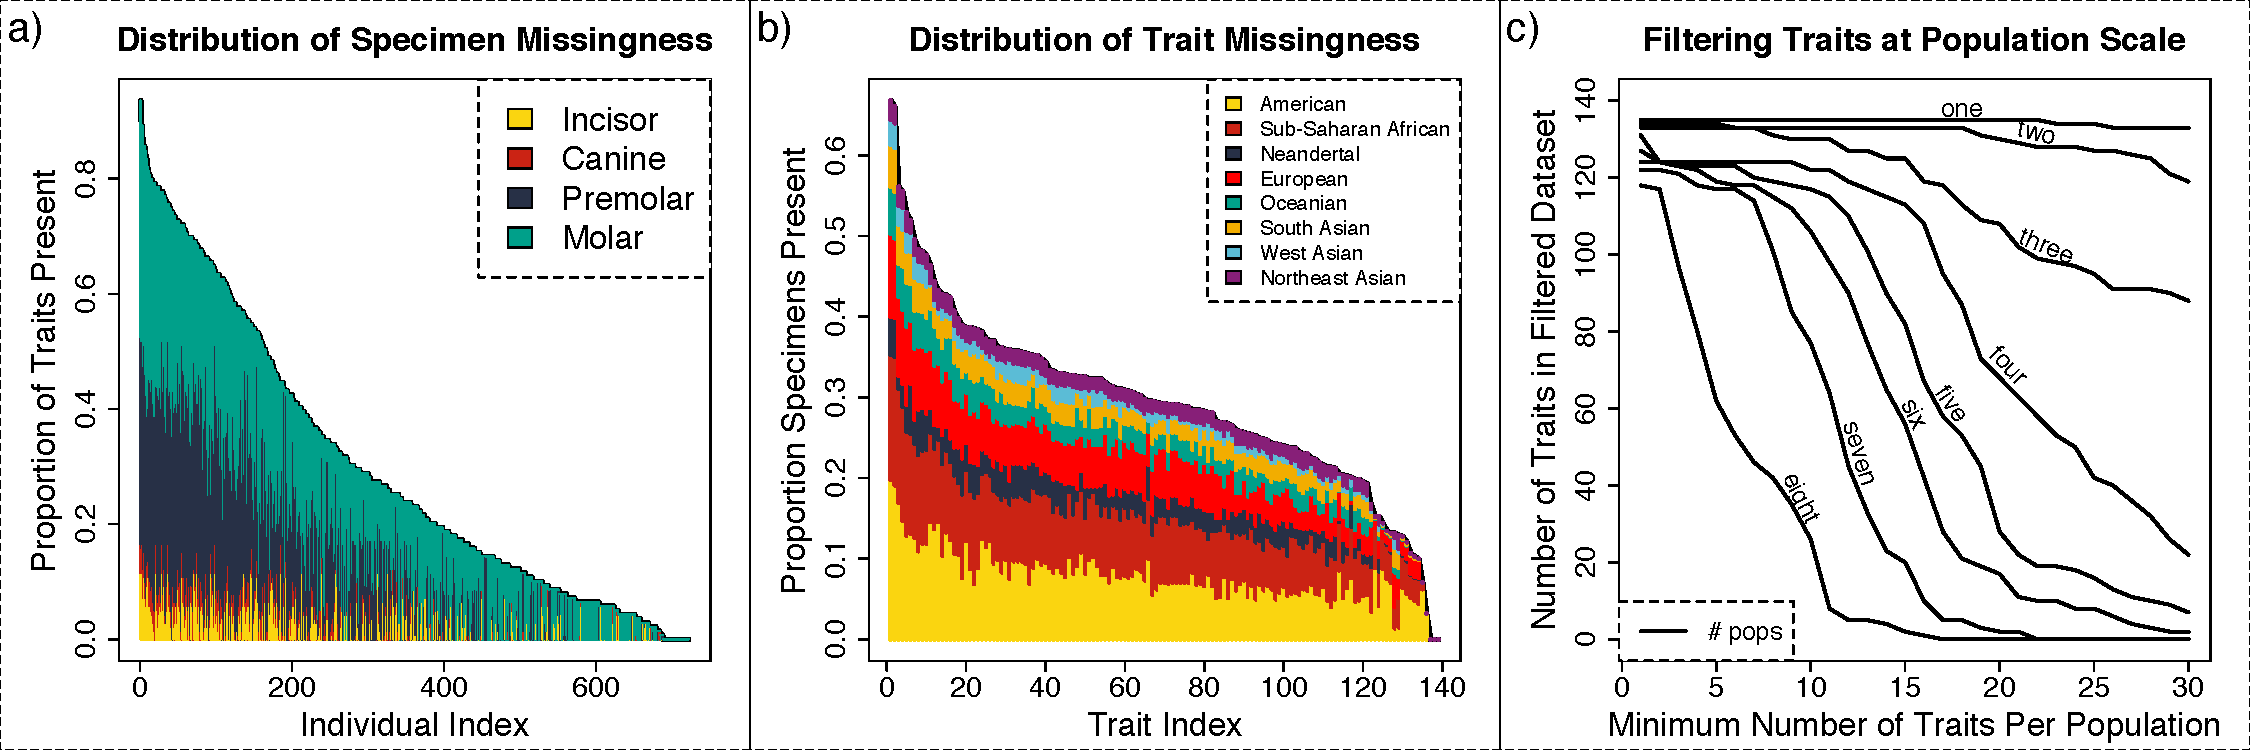
\includegraphics[width=160mm]{figures/bailey_figure1.pdf}
%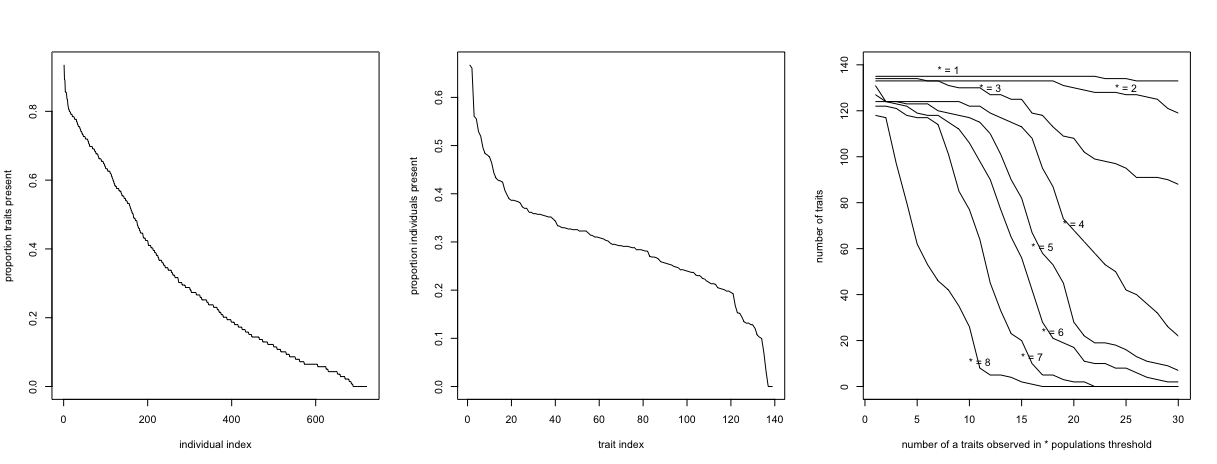
\includegraphics[width=180mm]{figures/chpt4_figure1.png}
\caption[Discrete Dental Missingness Visualization]{A visualization of missingness in the unfiltered dataset. In a), the proportion of traits present in the sorted, decreasing set of individuals represented in the sample. Colors represent different tooth types, stacked according to their mesio-distal progression within the dentition. In b), the number of individuals available to represent each set. Colors represent populations, stacked according to total population size. In c), information in these figures is combined to produce a graph depicting how criteria pertaining to the minimum number of individuals in a minimum number of populations affects the number of traits ultimately present in the sample. \label{overflow}
\label{fig:missingnessDENTAL}}
\end{figure*}

\begin{figure*}[h]
\centering
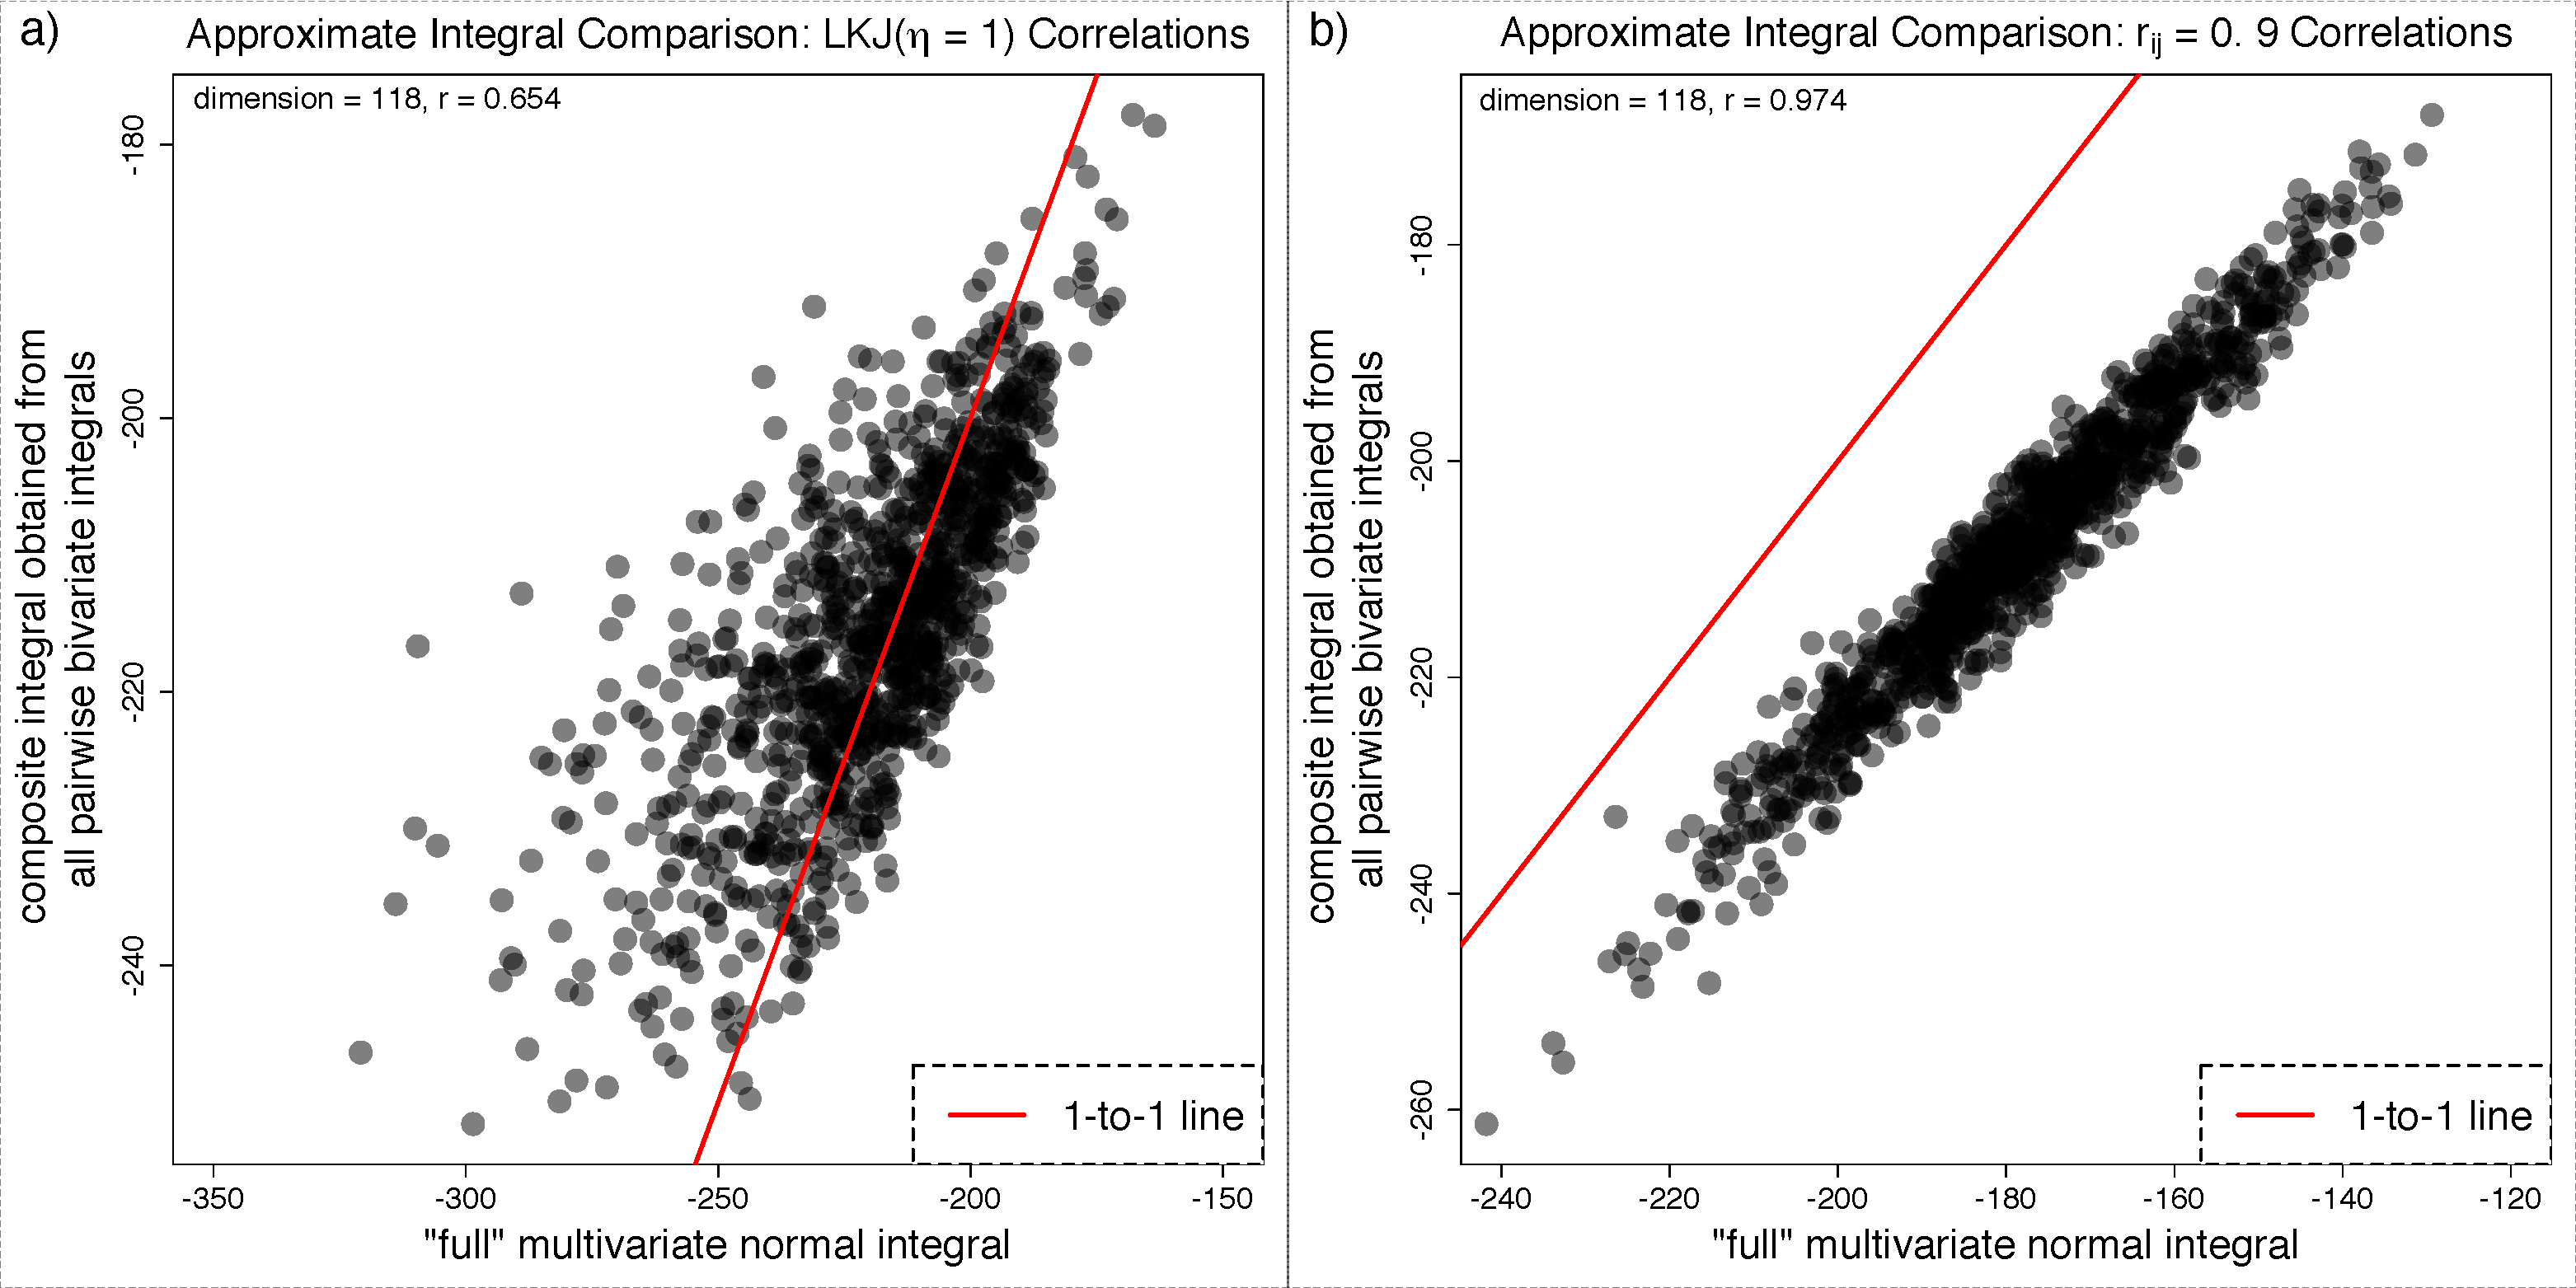
\includegraphics[width=160mm]{figures/chpt4_figure2.pdf}
\caption[Approximation of Multivariate Normal Integral by Bivariate Normal Integrals]{Visualizing relationships between the transformed bivariate integral of a multivariate normal and its full evaluation. In a), the integral of a multivariate normal with mean at the origin and 118 x 118 correlation matrix sampled from an LKJ(1) was evaluated with both methods between pairs of lower and upper bounds sampled at uniform and sorted from the (-1,1) range. The log$_e$ scale output of 1,000 such simulations is shown, with 1-to-1 line marked and correlation between the two labeled. In b), the procedure is repeated, except with the correlation matrix to have all off-diagonal elements equal to 0.9.  
\label{fig:bivVSmultivDENTAL}
\label{overflow}}
\end{figure*}

\begin{figure*}[h]
\centering
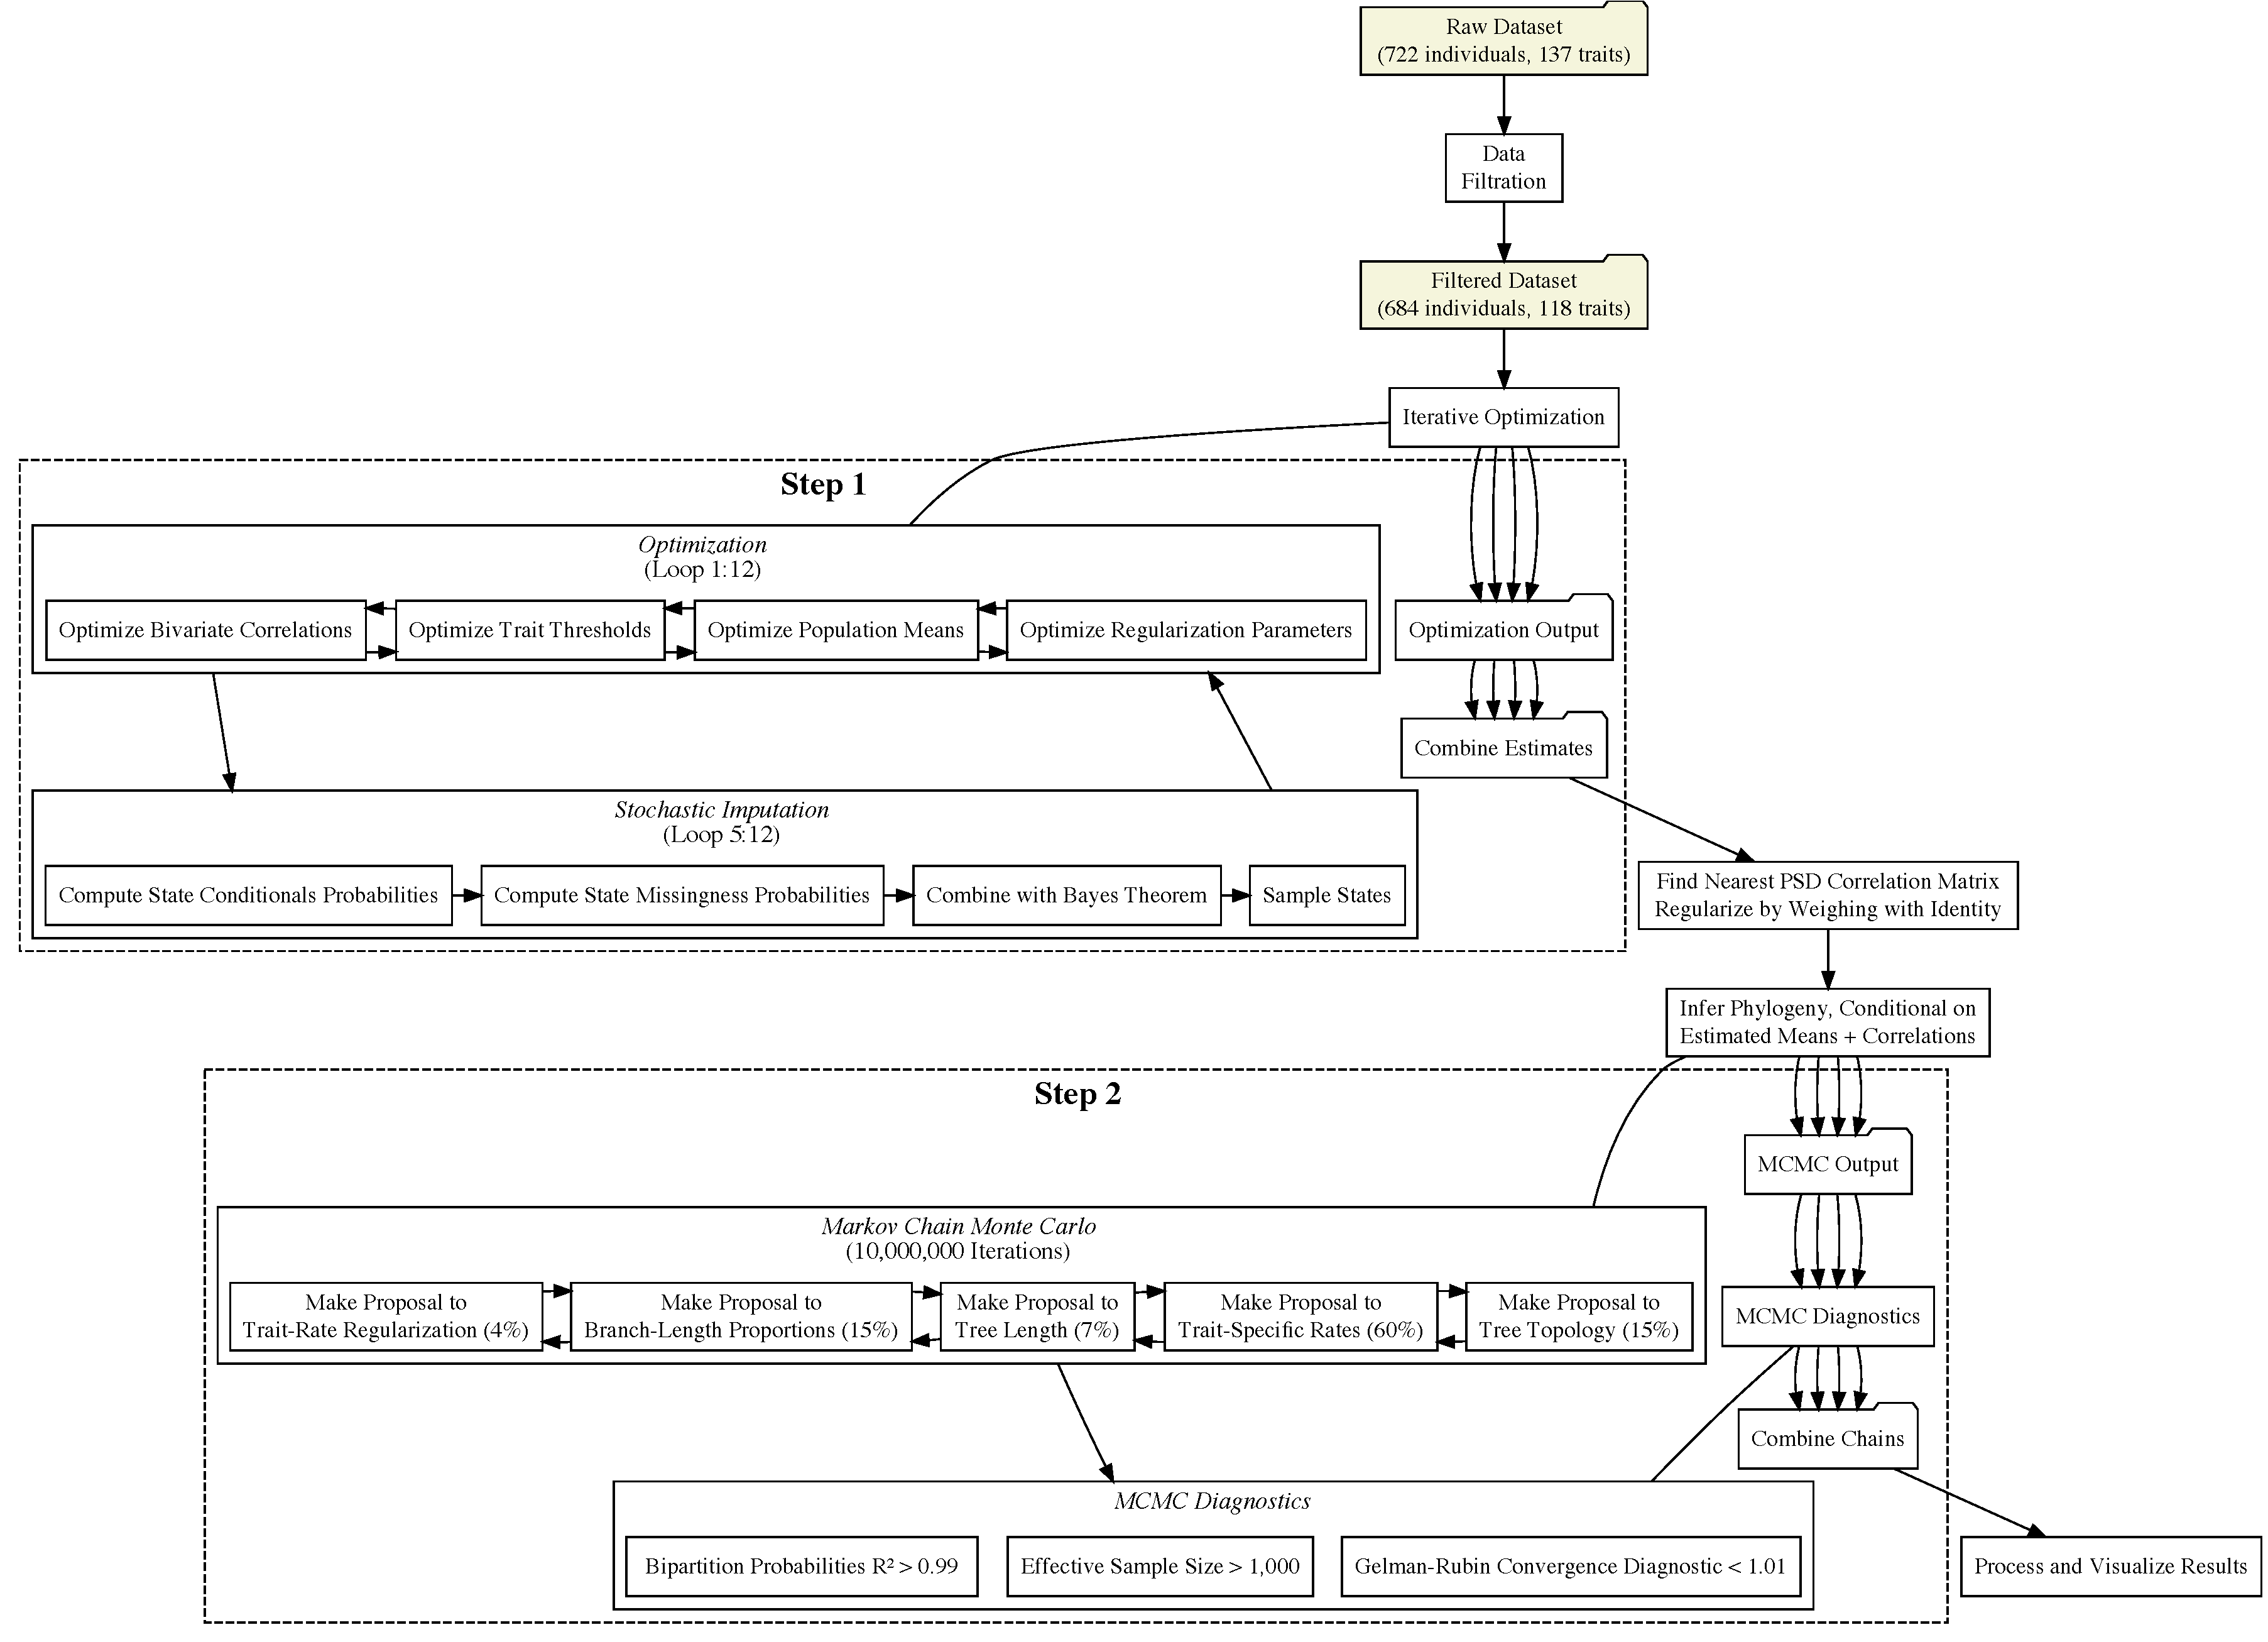
\includegraphics[width=160mm]{figures/tsarmbop.pdf}
\caption[TSAR-MBOP Flowchart]{A flowchart depicting the order of analysis and other data and output processing steps performed during the TSAR-MBOP procedure. \label{overflow}
\label{fig:tsarMBOP}
}
\end{figure*}

\begin{figure*}[h]
\centering
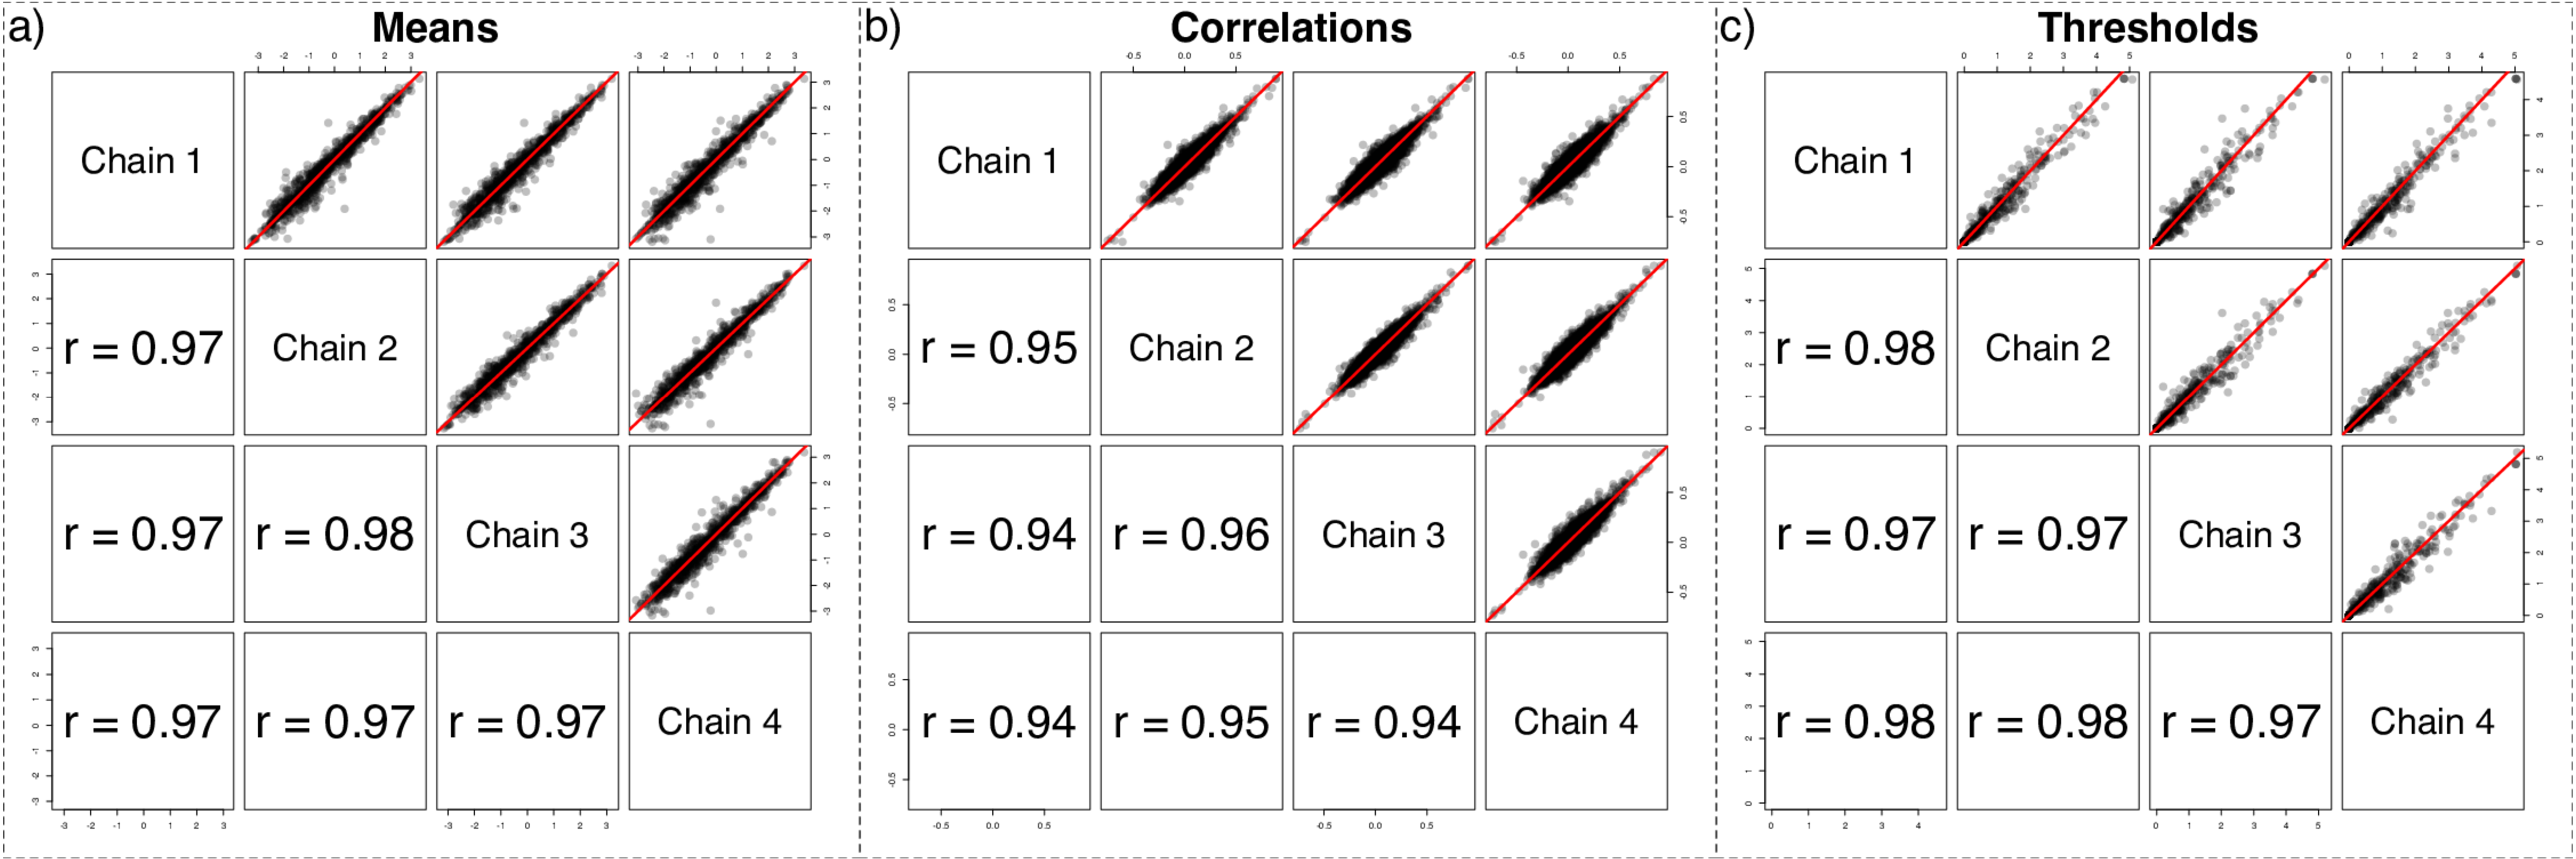
\includegraphics[width=160mm]{figures/chpt4_figure3.pdf}
\caption[Optimization Output from Four Runs of Discrete Dental Analysis]{Output from the iterative optimization step of our two-step algorithm across four independent runs. In a), means are plotted in the upper right panels of the figure, with correlations between runs in the lower left panels. In b), within-group, between-liability correlation parameters are plotted. In c), threshold locations.  
\label{fig:empiricalOptimOutput}
\label{overflow}}
\end{figure*}

\begin{figure*}[h]
\centering
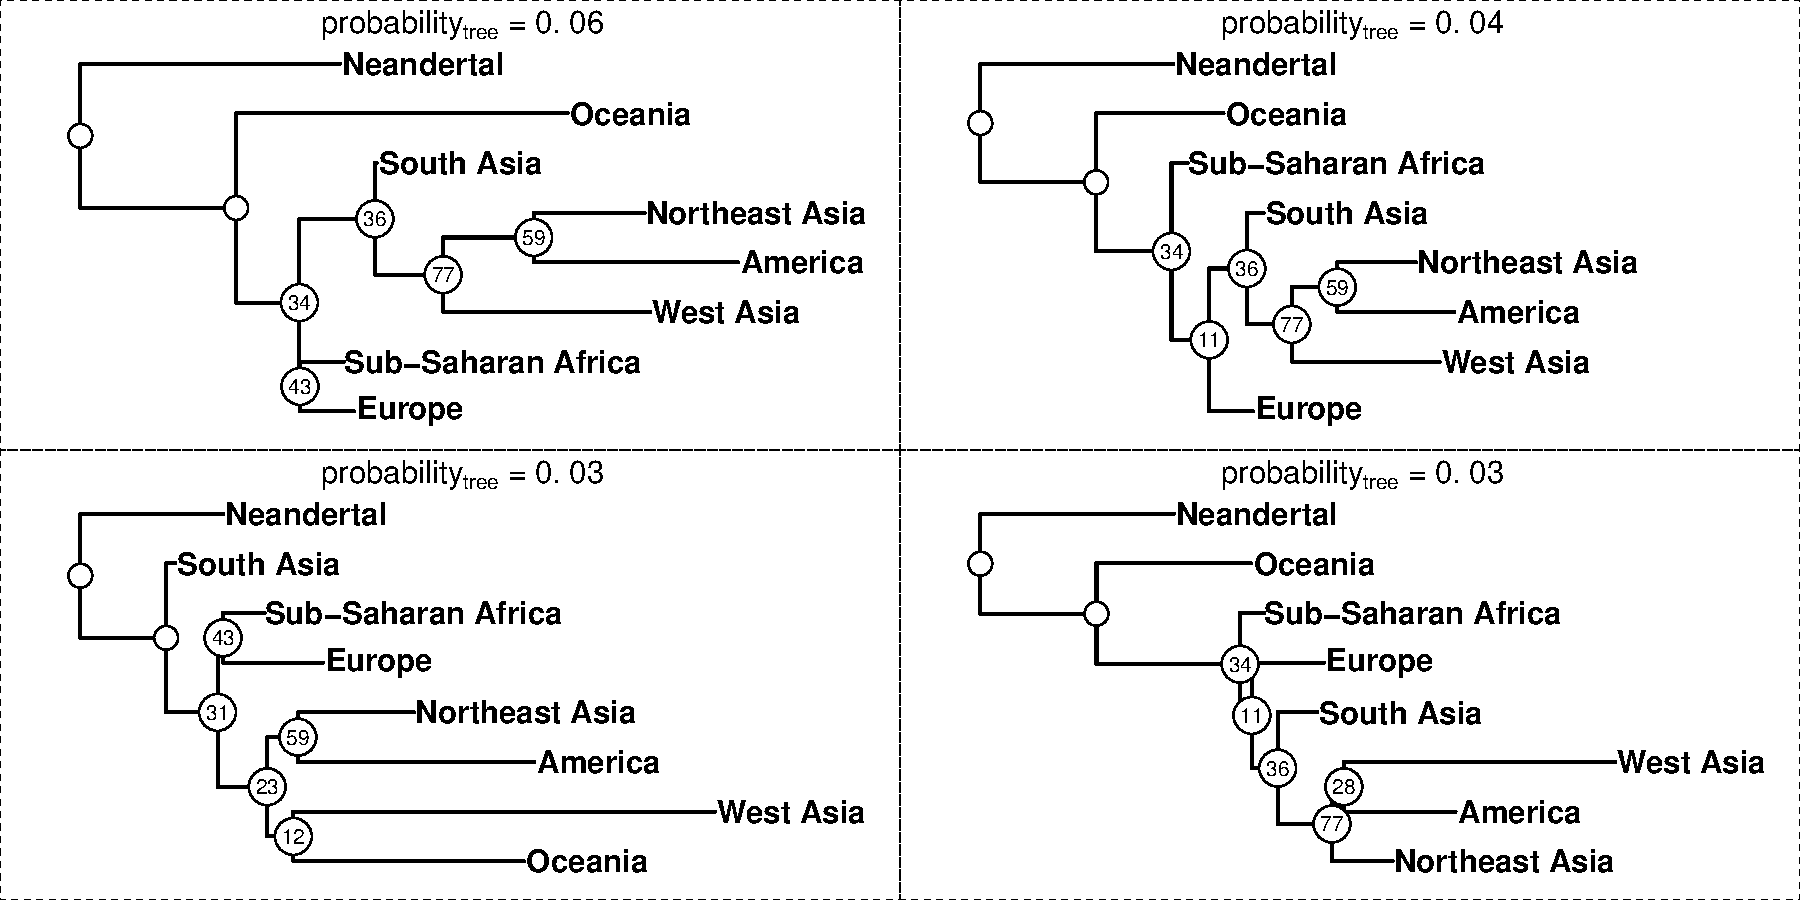
\includegraphics[width=160mm]{figures/dental_top4trees.pdf}
\caption[Top Four Tree Topologies from Discrete Dental Phylogenetic Analysis]{The four most probable trees from the posterior distribution of our Bayesian phylogenetic analysis, with nodal posterior probabilities plotted. Branch lengths are posterior mean estimates conditional on  each tree topology and are proportional to the extent of morphological evolution on each branch. Trees were rooted along the Neandertal branch approximately $\frac{5}{8}^{ths}$ of the length to the internal node.  
\label{overflow}
\label{fig:top4treesDENTAL}}
\end{figure*}

\begin{figure*}[h]
\centering
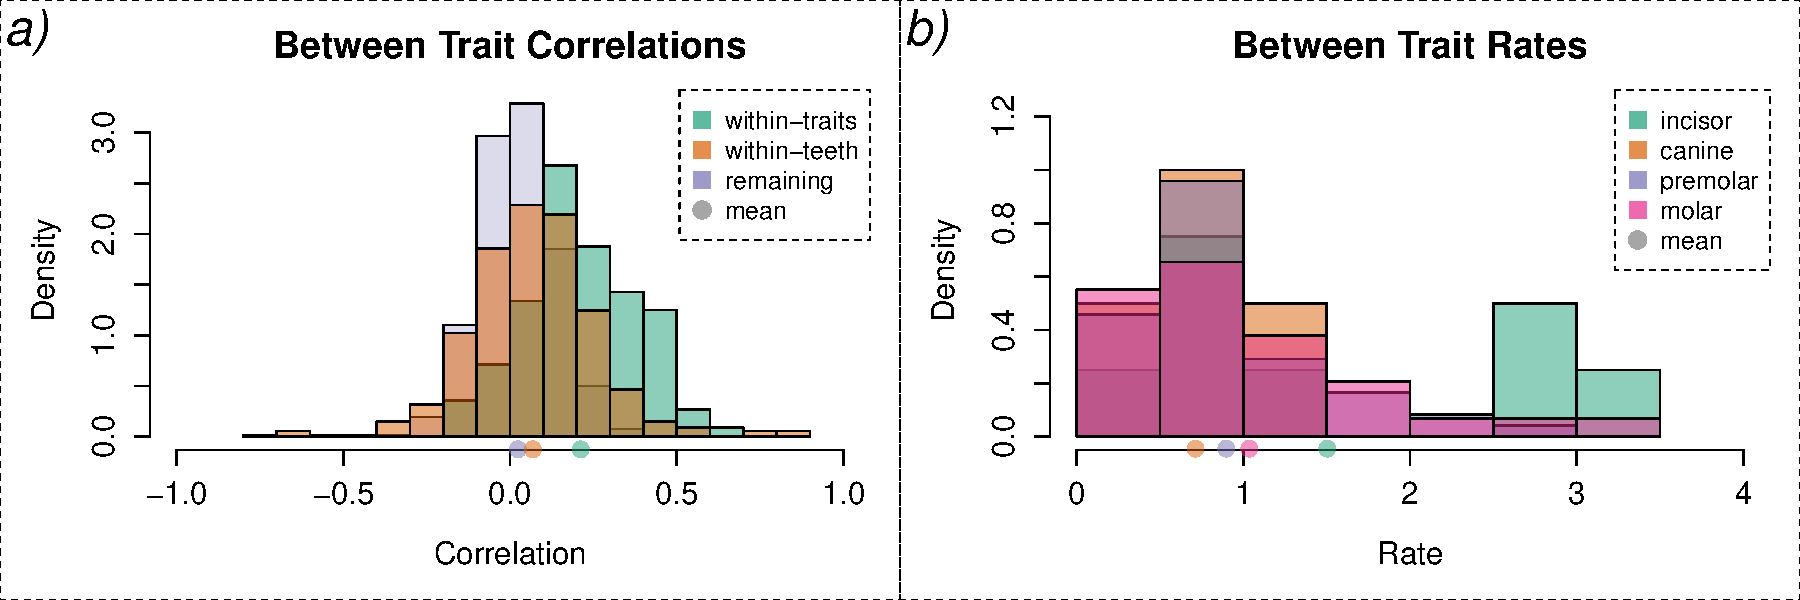
\includegraphics[width=160mm]{figures/dental_rates_corrs.pdf}
\caption[Estimated Rates and Correlations of Discrete Dental Evolution]{In a), histograms of correlations between traits within individual teeth, within traits across teeth, and for the remaining elements of the correlation matrix are plotted. Correlations are those from the evolutionary rate matrix, and so are interpretable as correlations of the evolutionary process, though they were estimated from within-population data per Cheverud's conjecture. In b) posterior means of trait-specific rates are partitioned across types of tooth within the human dentition, and tooth-specific histograms are plotted. Means in both panels are marked with color-coded filled circles. \label{overflow}
\label{fig:dentalRatesCorrs}
}
\end{figure*}


\begin{figure*}[h]
\centering
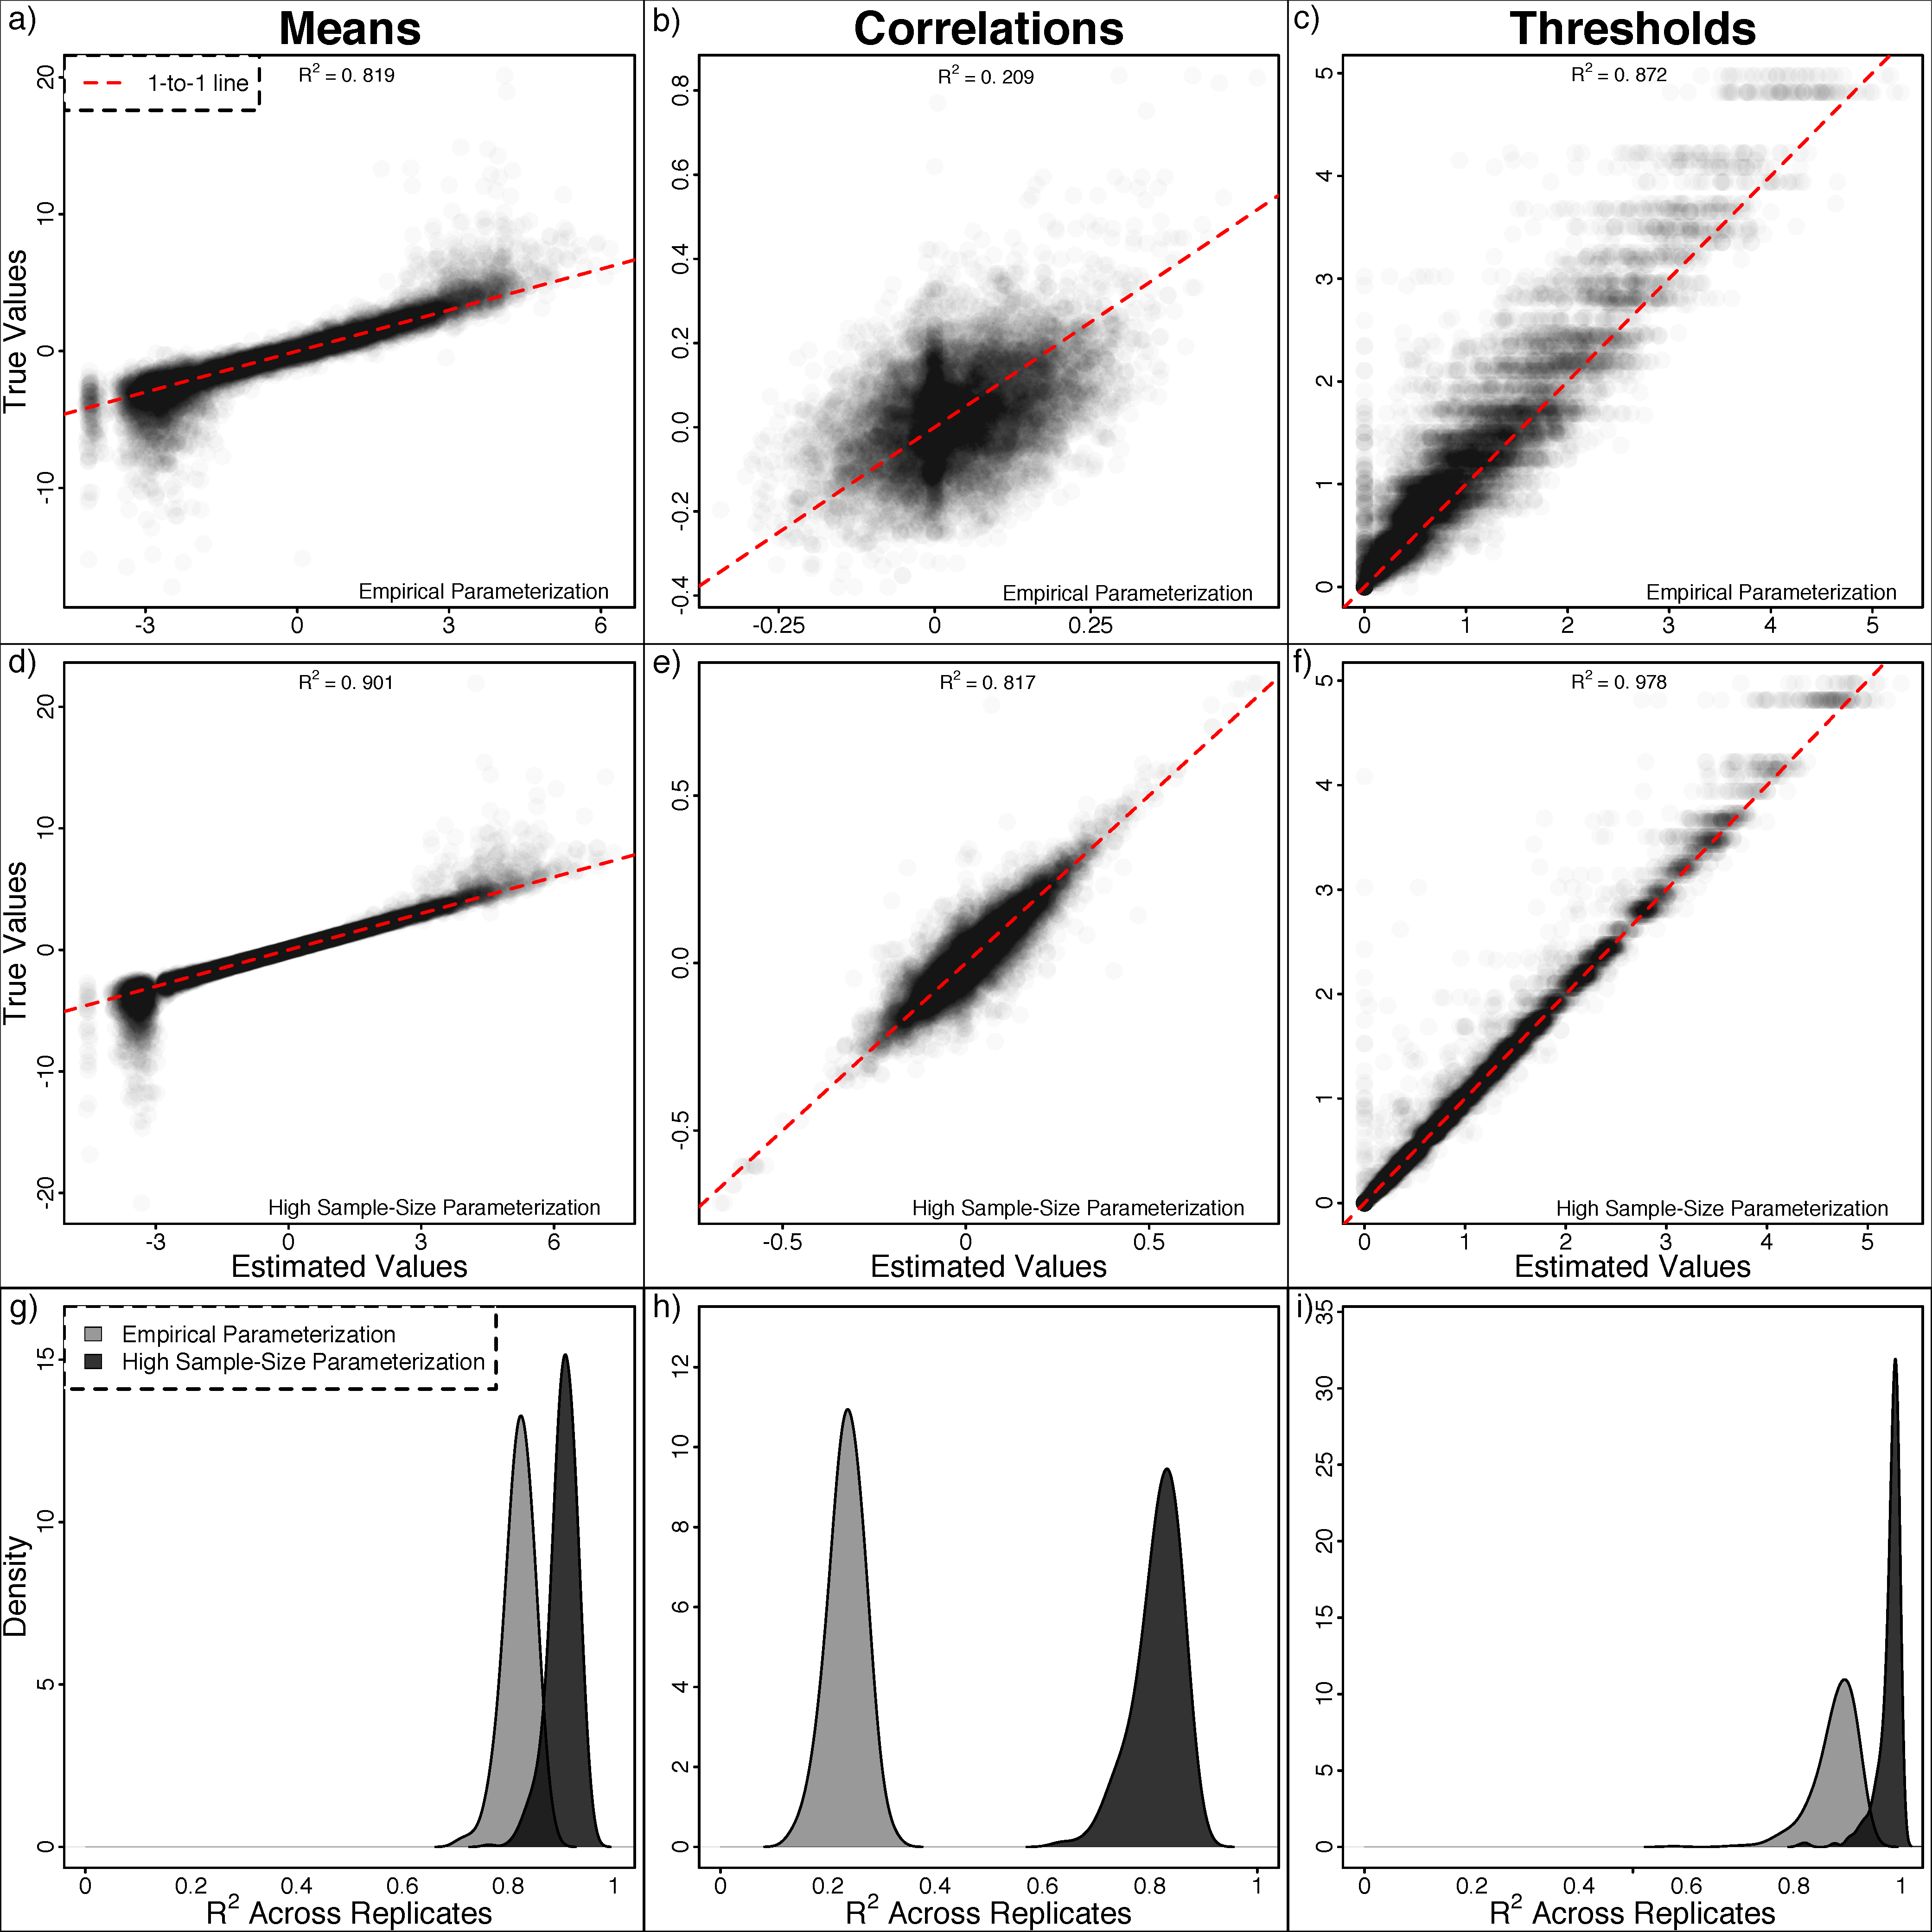
\includegraphics[width=160mm]{figures/chpt4_figure6.pdf}
\caption[Optimization Output for TSAR-MBOP Simulation Study]{In a-c), estimates of population means, between-trait / within-group correlations, and threshold locations, respectively, are plotted together for 500 simulations under the lower-sampled, empirically parameterized condition. The one-to-one line is shown, and an overall $R^2$ is labeled. In d-f), the same are plotted for the ``high-sample size'' condition. Finally, in g-i), kernel density estimates are plotted for both conditions for replicate-specific $R^2$ values.  \label{overflow}
\label{fig:simsOptimResults}
}
\end{figure*}


\begin{figure*}[h]
\centering
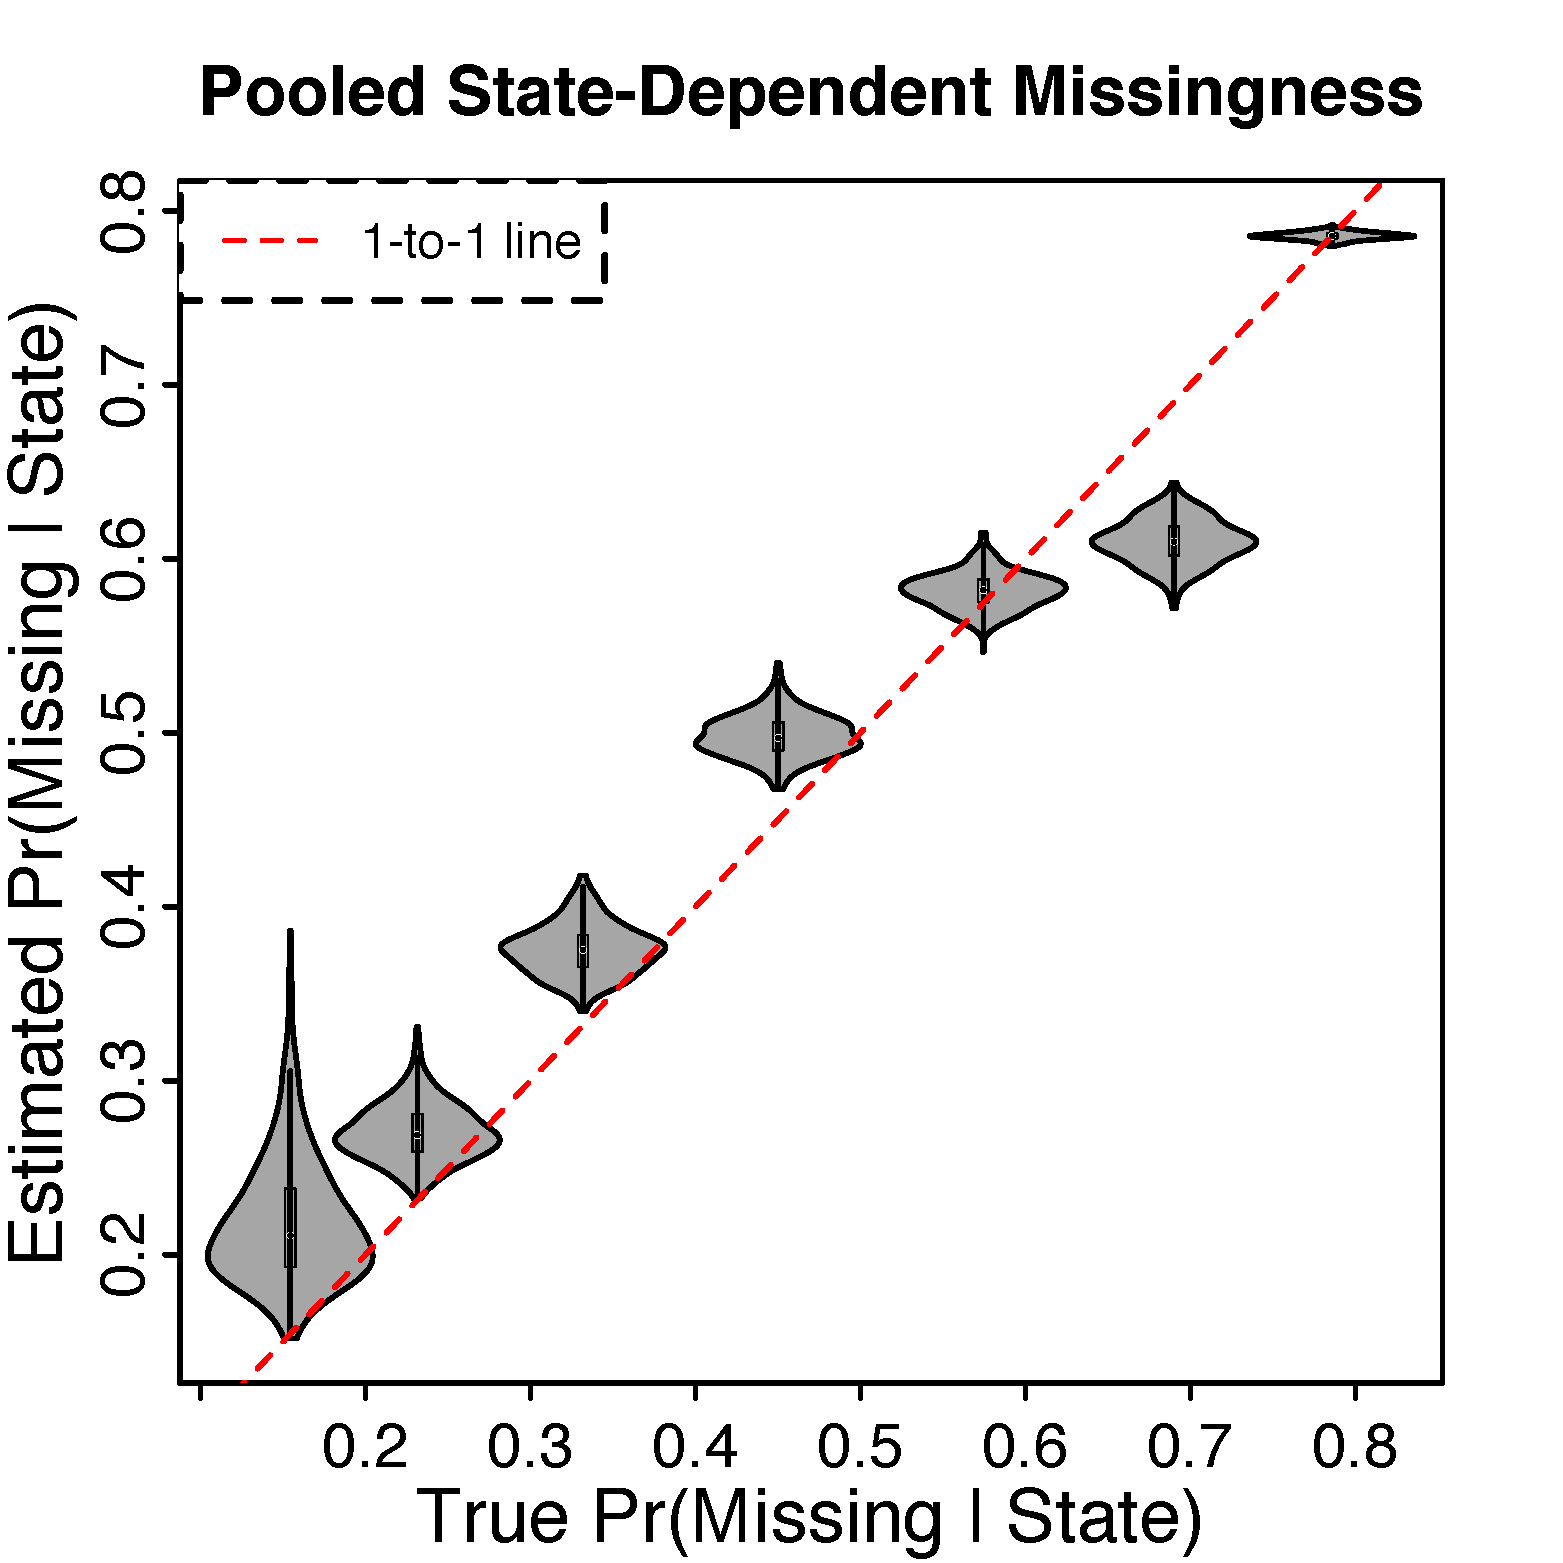
\includegraphics[width=160mm]{figures/chpt4_figure7.pdf}
\caption[Violin Plots of Estimated State-Dependent Missing Probabilities]{Estimates of state-dependent missingness during the last round of iterative optimization, averages across four independent chains. Violin plots show the distribution of these estimates across 500 replicate analyses of simulated data under the ``empirically parameterized'' condition. These estimates are pooled across traits for visual clarity, but analyses used trait-specific estimates as between-trait commensurability was questionable. A one-to-one line is plotted for ease of interpretation. \label{overflow}
\label{fig:simsMissingProbs}
}
\end{figure*}


\begin{figure*}[h]
\centering
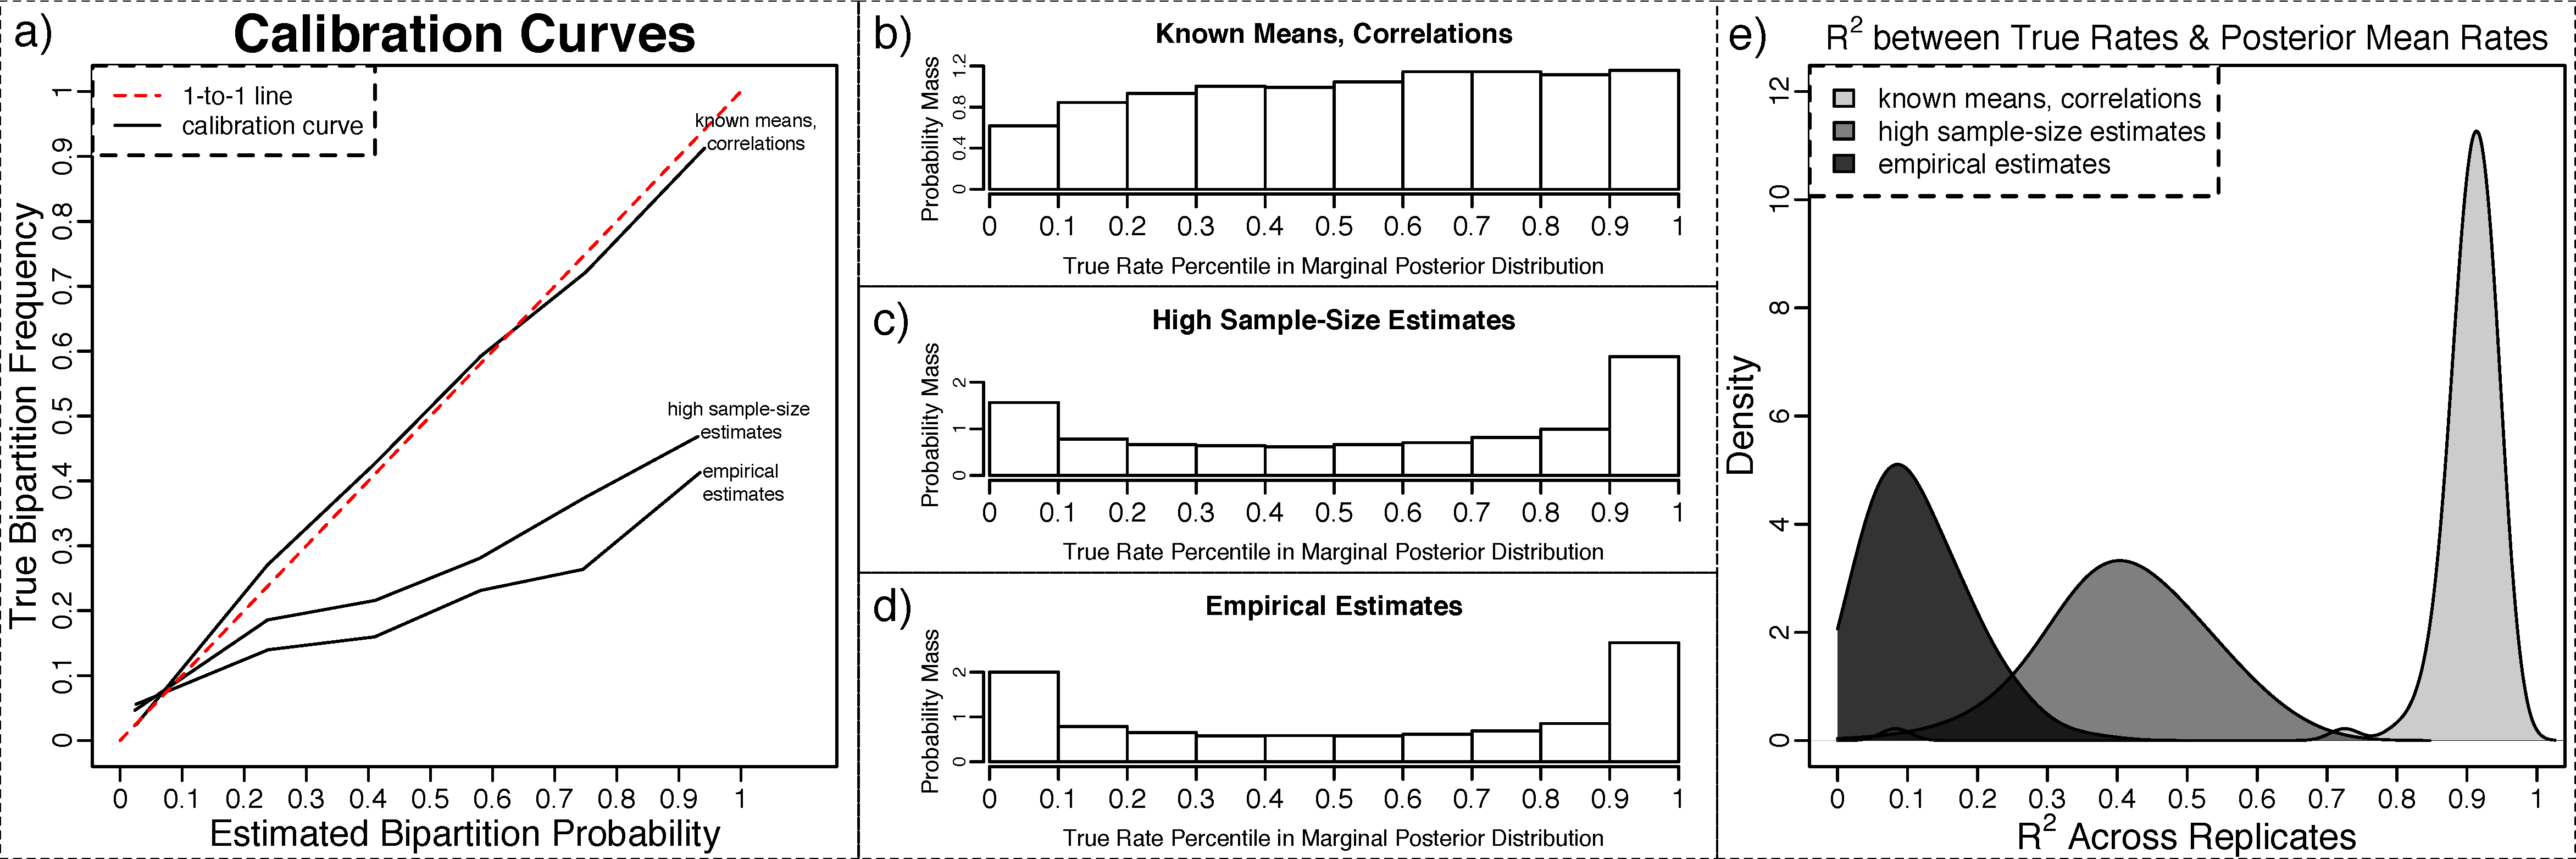
\includegraphics[width=160mm]{figures/chpt4_figure8.pdf}
\caption[Calibration Curves for TSAR-MBOP Simulation Study]{In a), calibration curves across the three sets of simulation conditions: where discrete data were simulated under conditions resembling our empirical dataset (labeled \textit{empirical estimates}), where it was simulated under high-sample size conditions described in text (labeled \textit{high sample-size estimates}, and where it was not simulated at all, and true means and correlations were used. These curves describe the relationship between an estimated bipartition probability and the true frequency with which it was found in the data-generating tree, with pooling done within sextiles. In b-d), percentile plots of true, data-generating trait-specific rates in the marginal posterior distribution for each of those rates are shown for each of the three conditions, with plot data pooled across replicates. In e), kernel density estimates of $R^2$ values between true-rates and the posterior means of these trait-specific rates are shown across replicates. \label{overflow}
\label{fig:simsCalibration}
}
\end{figure*}

\clearpage

\section{Tables}

% latex table generated in R 3.6.2 by xtable 1.8-4 package
% Wed Sep 30 14:43:13 2020
\begin{longtable}{rrrrrrrrr}
  \hline
 & NEAN & OCEAN & EUR & WAS & SAS & NEAS & SSAF & AMER \\ 
  \hline
UI1.LC &  25 &   9 &  37 &   5 &  16 &   8 &  37 &  54 \\ 
  UI1.SH &  26 &   9 &  36 &   5 &  12 &   9 &  36 &  39 \\ 
  UI1.DSH &  25 &   8 &  37 &   5 &  16 &   8 &  36 &  44 \\ 
  UI1.TD &  25 &  11 &  32 &   4 &   8 &   7 &  32 &  35 \\ 
  UI2.SH &  26 &  13 &  24 &   3 &  15 &  11 &  39 &  49 \\ 
  UI2.DSH &  22 &  13 &  26 &   3 &  19 &   9 &  40 &  42 \\ 
  UI2.IG &  22 &  16 &  17 &   3 &  15 &   8 &  36 &  36 \\ 
  UI2.TD &  19 &  15 &  24 &   3 &  11 &  10 &  38 &  41 \\ 
  C.SH &  22 &  12 &  26 &   6 &  13 &  10 &  43 &  53 \\ 
  C.DSH &  22 &  12 &  29 &   6 &  19 &  10 &  47 &  60 \\ 
  C.TD &  23 &  11 &  26 &   6 &  15 &   8 &  37 &  47 \\ 
  C.MR &  19 &  11 &  21 &   5 &  12 &   9 &  33 &  37 \\ 
  UPM3.BMR &  21 &  16 &  44 &   5 &  15 &   9 &  62 &  58 \\ 
  UPM3.LMR &  17 &  15 &  43 &   5 &  16 &   9 &  61 &  57 \\ 
  UPM3.BMRF &  19 &  16 &  44 &   5 &  13 &   9 &  62 &  56 \\ 
  UPM3.LMRF &  17 &  15 &  43 &   5 &  14 &   9 &  61 &  57 \\ 
  UPM3.TM &  24 &  19 &  45 &   6 &  21 &  12 &  64 &  88 \\ 
  UPM3.DAC &  20 &  16 &  40 &   5 &  20 &  11 &  65 &  64 \\ 
  UPM3.MAC &  20 &  16 &  43 &   6 &  20 &  12 &  62 &  69 \\ 
  UPM3.XC &  17 &  18 &  45 &   6 &  21 &  12 &  67 &  83 \\ 
  UPM4.BMR &  23 &  20 &  40 &   3 &  14 &  13 &  54 &  55 \\ 
  UPM4.LMR &  19 &  16 &  42 &   3 &  14 &  12 &  52 &  51 \\ 
  UPM4.BMRF &  20 &  19 &  42 &   3 &  13 &  13 &  52 &  53 \\ 
  UPM4.LMRF &  19 &  17 &  43 &   3 &  12 &  11 &  51 &  49 \\ 
  UPM4.TM &  22 &  23 &  44 &   4 &  20 &  14 &  58 &  90 \\ 
  UPM4.DAC &  20 &  19 &  39 &   3 &  16 &  11 &  48 &  63 \\ 
  UPM4.MAC &  20 &  21 &  35 &   3 &  14 &  12 &  52 &  61 \\ 
  UPM4.XC &  17 &  21 &  44 &   4 &  20 &  14 &  59 &  88 \\ 
  UM1.ME &  34 &  42 &  74 &  22 &  38 &  17 & 112 & 143 \\ 
  UM1.HY\_RED &  35 &  42 &  71 &  22 &  39 &  15 & 115 & 138 \\ 
  UM1.C5 &  22 &  34 &  63 &  20 &  30 &  14 &  84 &  91 \\ 
  UM1.CC &  24 &  39 &  70 &  19 &  28 &  16 &  93 &  93 \\ 
  UM1.EE &  21 &  39 &  66 &  19 &  33 &  15 & 102 & 106 \\ 
  UM1.BG &  12 &  29 &  71 &  17 &  35 &  17 & 102 & 122 \\ 
  UM1.MPT &  12 &  12 &  41 &   9 &  18 &   6 &  60 &  37 \\ 
  UM1.MAT &  12 &  14 &  40 &   8 &  17 &   5 &  60 &  37 \\ 
  UM1.PROT &  11 &  14 &  39 &   8 &  18 &   6 &  60 &  38 \\ 
  UM2.ME &  22 &  36 &  53 &   2 &  21 &  16 &  80 & 105 \\ 
  UM2.HY &  24 &  26 &  41 &   3 &  12 &  12 &  72 &  64 \\ 
  UM2.C5 &  21 &  37 &  54 &   5 &  16 &  14 &  70 &  89 \\ 
  UM2.CC &  21 &  35 &  53 &   5 &  19 &  16 &  72 &  99 \\ 
  UM2.EE &  21 &  30 &  51 &   5 &  18 &  14 &  73 &  96 \\ 
  UM2.BG &  12 &  24 &  56 &   4 &  21 &  16 &  74 & 105 \\ 
  UM2.MPT &  10 &  25 &  44 &   3 &  13 &  11 &  55 &  65 \\ 
  UM2.MAT &  10 &  28 &  46 &   3 &  13 &  10 &  59 &  66 \\ 
  UM2.PROT &   9 &  27 &  44 &   3 &  12 &  10 &  57 &  71 \\ 
  UM3.ME &  13 &  13 &  17 &   4 &  16 &  12 &  43 &  40 \\ 
  UM3.HY &  17 &  15 &  17 &   4 &  18 &  13 &  37 &  45 \\ 
  UM3.C5 &  16 &  19 &  19 &   4 &  17 &  13 &  42 &  45 \\ 
  UM3.CC &  12 &  19 &  17 &   4 &  15 &  12 &  43 &  44 \\ 
  UM3.PA &  17 &  20 &  17 &   4 &  17 &  11 &  44 &  48 \\ 
  UM3.EE &  10 &  19 &  14 &   4 &  13 &   9 &  40 &  34 \\ 
  UM3.BG &  11 &   9 &  15 &   4 &  16 &  13 &  41 &  47 \\ 
  UM3.MPT &   7 &  16 &  18 &   4 &  14 &  10 &  31 &  46 \\ 
  UM3.MAT &   7 &  16 &  18 &   4 &  15 &  10 &  29 &  40 \\ 
  UM3.PROT &   9 &  15 &  18 &   4 &  16 &  10 &  30 &  39 \\ 
  UM3.PEG &  13 &  13 &  22 &   0 &  17 &  13 &  52 &  41 \\ 
  LP3.PLC &  31 &  16 &  37 &  16 &  20 &  11 &  59 &  71 \\ 
  LP3.AF &  23 &  17 &  36 &  15 &  15 &  11 &  56 &  65 \\ 
  LP3.MP &  29 &  18 &  36 &  16 &  20 &  11 &  58 &  70 \\ 
  LP3.MI &  28 &  18 &  37 &  16 &  20 &  11 &  58 &  68 \\ 
  LP3.MH &  29 &  17 &  37 &  16 &  20 &  11 &  58 &  70 \\ 
  LP3.XC &  28 &  17 &  36 &  16 &  20 &  11 &  59 &  70 \\ 
  LP3.LF &  29 &  18 &  37 &  16 &  20 &  11 &  57 &  71 \\ 
  LP3.DAR &  18 &  16 &  31 &  14 &  14 &  11 &  51 &  50 \\ 
  LP3.MAR &  14 &  16 &  35 &  13 &  17 &  11 &  54 &  50 \\ 
  LP3.MLG &  25 &  16 &  36 &  16 &  19 &  11 &  59 &  72 \\ 
  LP3.MeLG &   5 &  16 &  37 &  16 &  19 &   8 &  58 &  74 \\ 
  LP3.DLG &   8 &  16 &  37 &  16 &  19 &   8 &  58 &  74 \\ 
  LP3.ASM &  17 &  15 &  32 &   7 &  19 &  11 &  56 &  78 \\ 
  LP3.DLC &  15 &  16 &  37 &  12 &  20 &  11 &  56 &  66 \\ 
  LP4.PLC &  29 &  16 &  36 &  14 &  20 &  10 &  53 &  60 \\ 
  LP4.AF &  22 &  17 &  35 &  15 &  19 &   9 &  52 &  55 \\ 
  LP4.MP &  29 &  16 &  36 &  15 &  20 &  10 &  54 &  60 \\ 
  LP4.MI &  27 &  17 &  36 &  14 &  20 &  10 &  53 &  59 \\ 
  LP4.MH &  27 &  17 &  36 &  14 &  19 &   9 &  53 &  58 \\ 
  LP4.XC &  29 &  18 &  36 &  14 &  20 &  10 &  54 &  56 \\ 
  LP4.LF &  28 &  18 &  36 &  14 &  20 &  10 &  50 &  59 \\ 
  LP4.DAR &  14 &  13 &  33 &   9 &  14 &   8 &  48 &  36 \\ 
  LP4.MAR &  15 &  13 &  32 &   9 &  17 &   9 &  51 &  36 \\ 
  LP4.MLG &  25 &  10 &  35 &  15 &  20 &   8 &  32 &  58 \\ 
  LP4.ASM &  30 &  10 &  30 &   9 &   0 &   8 &  54 &  72 \\ 
  LM1.4CUS &  45 &  33 &  56 &  17 &  29 &  11 &  89 &  95 \\ 
  LM1.DW &  25 &  14 &  37 &  10 &  14 &   7 &  60 &  45 \\ 
  LM1.DTC &  31 &  26 &  47 &  12 &  26 &   9 &  77 &  50 \\ 
  LM1.MTC &  32 &  27 &  46 &  12 &  24 &  10 &  75 &  55 \\ 
  LM1.PR &  38 &  31 &  55 &  17 &  27 &  10 &  83 &  86 \\ 
  LM1.C5 &  41 &  32 &  56 &  17 &  27 &  11 &  86 &  79 \\ 
  LM1.C6 &  21 &  22 &  49 &  16 &  21 &   9 &  67 &  54 \\ 
  LM1.C7 &  32 &  30 &  56 &  17 &  28 &  11 &  84 &  86 \\ 
  LM1.EE &  26 &  30 &  48 &  11 &  26 &  11 &  82 &  75 \\ 
  LM1.AF &  33 &  18 &  40 &  13 &  18 &   9 &  74 &  50 \\ 
  LM2.DW &  19 &  25 &  37 &   9 &  17 &  10 &  59 &  51 \\ 
  LM2.DTC &  26 &  32 &  43 &  11 &  21 &  13 &  70 &  63 \\ 
  LM2.MTC &  25 &  33 &  43 &  11 &  21 &  13 &  67 &  64 \\ 
  LM2.PR &  32 &  31 &  42 &  12 &  17 &  13 &  64 &  76 \\ 
  LM2.C5 &  27 &  30 &  40 &  11 &  17 &  11 &  65 &  60 \\ 
  LM2.C6 &  18 &  23 &  40 &  11 &  17 &  10 &  54 &  40 \\ 
  LM2.C7 &  25 &  33 &  43 &  12 &  21 &  13 &  70 &  77 \\ 
  LM2.EE &  18 &  27 &  38 &   8 &  17 &  13 &  63 &  67 \\ 
  LM2.AF &  22 &  31 &  40 &  10 &  20 &  11 &  65 &  68 \\ 
  LM3.4CUS &   0 &   8 &  19 &   3 &  14 &  12 &  26 &  11 \\ 
  LM3.DW &  14 &  18 &  17 &   6 &  12 &  12 &  46 &  29 \\ 
  LM3.DTC &  18 &  21 &  19 &   7 &  16 &  12 &  53 &  38 \\ 
  LM3.MTC &  16 &  21 &  19 &   7 &  16 &  12 &  52 &  44 \\ 
  LM3.PR &  21 &  23 &  16 &   7 &  14 &  11 &  44 &  50 \\ 
  LM3.C5 &  14 &  21 &  19 &   5 &  13 &  11 &  52 &  48 \\ 
  LM3.C6 &   9 &  21 &  19 &   5 &  14 &  11 &  50 &  42 \\ 
  LM3.C7 &  15 &  22 &  18 &   7 &  16 &  12 &  48 &  56 \\ 
  LM3.EE &  11 &  13 &  14 &   3 &  12 &   9 &  46 &  35 \\ 
  LM3.AF &  14 &  19 &  15 &   7 &  14 &  12 &  46 &  40 \\ 
  UPM3.BMxP\_MR &  18 &  14 &  42 &   4 &  13 &   8 &  60 &  51 \\ 
  UPM3.BMxP\_DR &  18 &  14 &  42 &   4 &  13 &   8 &  60 &  51 \\ 
  UPM3.LMxP\_MR &  17 &  13 &  44 &   5 &  13 &   8 &  60 &  51 \\ 
  UPM3.LMxP\_DR &  17 &  13 &  44 &   5 &  13 &   8 &  60 &  51 \\ 
  UPM4.LMxP\_MR &  18 &  17 &  42 &   3 &  14 &  12 &  49 &  48 \\ 
  UPM4.LMxP\_DR &  18 &  17 &  42 &   3 &  14 &  12 &  50 &  48 \\ 
  UPM4.BMxP\_MR &  17 &  19 &  40 &   3 &  14 &  11 &  53 &  51 \\ 
   \hline
\hline
\caption[Composition of Dental Data Used in Empirical Analysis]{A table detailing the composition of the discrete dental data used in 
                                     our empirical analysis. Elements of the table represent numbers of individuals in each 
                                     column population with a definitive observation in each 
                                     row trait. Population codes are as follow: NEAN (\textit{Neandertal}), OCEAN (\textit{Oceanian}), EUR (\textit{European}), WAS (\textit{West Asian}), SAS (\textit{South Asian}), NEAS (\textit{Northeast Asian}), SSAF (\textit{Sub-Saharan African}), AMER (\textit{American}). Details regarding trait codes key can be found in \citep{baileyNeandertalDentalMorphology2002}.} 
\label{tab:dentalDataComposition}
\end{longtable}


\clearpage

\section{Supplemental Figures}

\label{supp:SupplementalFiguresThresholdModel}

\begin{figure*}[h]
\centering
\includemovie[
  poster={anime/univ_threshold_mu_smooth.png}]{16cm}{5.6cm}{anime/univ_threshold_mu_smooth.mp4}
\caption[Varying the Location of a Population Mean Under the Univariate Threshold Model]{Visualizing the effect of smooth variation in a univariate mean liability on the ordinal trait frequencies of a hypothetical population. MP4 viewable with a compatible PDF Reader.}
\label{fig:univMuSmooth}
\end{figure*}

\begin{figure*}[h]
\centering
\includemovie[
  poster={anime/univ_threshold_thresh_smooth.png}]{16cm}{5.6cm}{anime/univ_threshold_thresh_smooth.mp4}
\caption[Varying the Location of a Threshold Under the Univariate Threshold Model]{Visualizing the effect of smooth variation in the location of a threshold on the ordinal trait frequencies of a hypothetical population. MP4 viewable with a compatible PDF Reader.}
\label{fig:univThreshSmooth}
\end{figure*}

\begin{figure*}[h]
\centering
\includemovie[
  poster={anime/univThresh_meanWiggle.png}]{16cm}{4.05cm}{anime/univThresh_meanWiggle.mp4}
\caption[Univariate Brownian Motion Under the Threshold Model]{Visualizing the effect of a univariate Brownian motion process acting on a univariate mean liability on the ordinal trait frequencies of a hypothetical population. MP4 viewable with a compatible PDF Reader.}
\label{fig:univThreshMeanWiggle}
\end{figure*}

\begin{figure*}[h]
\centering
\includemovie[
  poster={anime/mv_mu_both.png}]{16cm}{8.763cm}{anime/mv_mu_both.mp4}
\caption[Varying the Location of a Population Mean Under the Bivariate Threshold Model]{Visualizing the effect of smooth variation in a bivariate mean liability on the ordinal trait frequencies of a hypothetical population. MP4 viewable with a compatible PDF Reader.}
\label{fig:bivMuSmooth}
\end{figure*}

\begin{figure*}[h]
\centering
\includemovie[
  poster={anime/mv_thresh_both.png}]{16cm}{8.763cm}{anime/mv_thresh_both.mp4}
\caption[Varying the Location of Two Thresholds Under the Bivariate Threshold Model]{Visualizing the effect of smooth variation in  the locations of two thresholds on the ordinal trait frequencies of a hypothetical population. MP4 viewable with a compatible PDF Reader.}
\label{fig:bivThreshSmooth}
\end{figure*}

\begin{figure*}[h]
\centering
\includemovie[
  poster={anime/mv_corr_both.png}]{16cm}{8.763cm}{anime/mv_corr_both.mp4}
\caption[Varying the Location of a Correlation Coefficient Under the Bivariate Threshold Model]{Visualizing the effect of smooth variation in a correlation coefficient describing the non-independent expression of two traits on the ordinal trait frequencies of a hypothetical population. MP4 viewable with a compatible PDF Reader.}
\label{fig:bivCorrSmooth}
\end{figure*}

\begin{figure*}[h]
\centering
\includemovie[
  poster={anime/mv_mu_bm.png}]{16cm}{5.842cm}{anime/mv_mu_bm.mp4}
\caption[Bivariate Brownian Motion Under the Threshold Model]{Visualizing the effect of a bivariate Brownian motion process acting on a bvariate mean liability on the ordinal trait frequencies of a hypothetical population. MP4 viewable with a compatible PDF Reader.}
\label{fig:bivBM}
\end{figure*}

%   \begin{frame}[plain]
%      \begin{tikzpicture}[remember picture,overlay]
%         \node[anchor=south west, inner sep=0pt] at (current page.south west) {%
%           \movie[height = \paperheight, width = \paperwidth, poster, showcontrols] {}{figures/univThresh_meanWiggle.mp4}%
%         };
%      \end{tikzpicture}
%   \end{frame}


%\begin{frame}{Movie using media9}
%      \begin{figure}[!htb]
%        \movie[label=show3,%
%               width=1.0\textwidth,%
%               poster,%
%               % autostart,%
%               showcontrols,%
%               % loop,%
%              ]{\includegraphics[width=1.0\textwidth]
%               {figures/chpt4_figure5.png}}
%               {figures/univThresh_meanWiggle.mp4}
%        \caption{A media9 package movie embedded in PDF, using mp4 format.}
%      \end{figure}
%    \end{frame}



%\begin{figure}[!htb]
%\includemedia[
%  %activate=onclick, % default
%  addresource=figures/univThresh_meanWiggle.mp4
%  flashvars={
%    source=figures/univThresh_meanWiggle.mp4
%    &autoPlay=true % start playing on activation
%    &loop=true
%  },
%  passcontext %show player's right-click menu
%]{\includegraphics[height=0.45\linewidth]{samplePicture.eps}}{VPlayer9.swf}
%\caption{A media9 package movie embedded in PDF, using mp4 format.}
%\label{mov:ex3d}
%\end{figure}

%\includemedia[
%  width=\paperwidth,height=0.7\linewidth,
%  activate=pageopen,
%  addresource=figures/univThresh_meanWiggle.mp4,
%  flashvars={source=figures/univThresh_meanWiggle.mp4&autoPlay=true}
%]{}{VPlayer.swf}

%\begin{figure}[ht]
%\includemovie{16cm}{6cm}{figures/univThresh_meanWiggle.mp4}
%\end{figure}


%    \begin{frame}{Movie using media9}
%      \begin{figure}[!htb]
%        \movie[label=show3,%
%               width=1.0\textwidth,%
%               poster,%
%               % autostart,%
%               showcontrols,%
%               % loop,%
%              ]{\includegraphics[width=1.0\textwidth]
%               {figures/middle_burst.png}}
%               {figures/univThresh_meanWiggle.mp4}
%        \caption{A media9 package movie embedded in PDF, using mp4 format.}
%      \end{figure}
%    \end{frame}
%    \label{mov:show3}


%\includemedia[
%  width=0.4\linewidth,
%  height=0.3\linewidth,
%  activate=pageopen,
%  addresource=figures/univThresh_meanWiggle.mp4,
%  flashvars={source=figures/univThresh_meanWiggle.mp4}
%]{}{VPlayer.swf}

%\begin{figure*}[h]
%\centering
%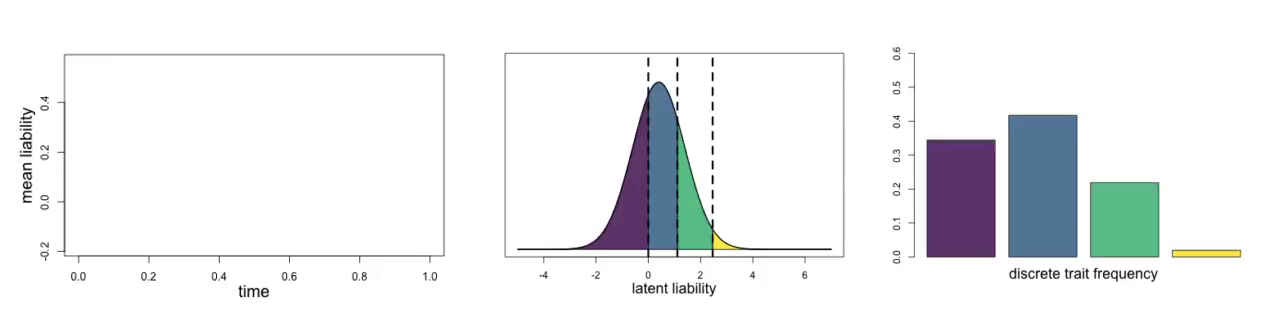
\includegraphics[width=160mm]{figures/univThresh_meanWiggle.mp4}
%%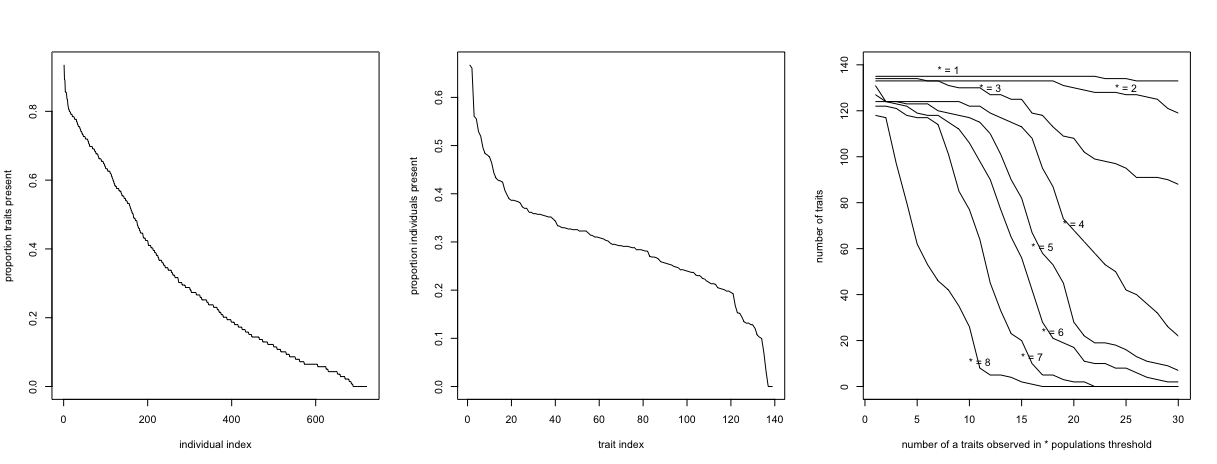
\includegraphics[width=160mm]{figures/chpt4_figure1.png}
%\caption{An animation of the evolution of a population mean liability according to the univariate Brownian motion process. Conditional on an ordered set of threshold locations, some proportion of discrete characters results. \label{overflow}
%\label{fig:univThreshMeanWiggle}}
%\end{figure*}

\clearpage

\twocolumn
%\nocite{*}
\bibliographystyle{apalike}
{
\footnotesize
\bibliography{plosone_paper_references.bib}
}

\end{document}
